\documentclass[11pt,letterpaper]{article}
\usepackage[margin=1in,headheight=15pt]{geometry}
\usepackage{fontspec}
\setmainfont{lmroman10-regular.otf}[BoldFont=lmroman10-bold.otf,ItalicFont=lmroman10-italic.otf,BoldItalicFont=lmroman10-bolditalic.otf]
\setsansfont{DejaVu Sans}[Scale=MatchLowercase]
\setmonofont{DejaVu Sans Mono}[Scale=0.82]
\usepackage{amsmath,amsthm,mathtools}
\usepackage{unicode-math}
\setmathfont{latinmodern-math.otf}
\usepackage{microtype}
\usepackage{booktabs,longtable,array,tabularx}
\usepackage{enumitem}
\usepackage{fvextra}
\usepackage[most]{tcolorbox}
\usepackage{tikz}
\usetikzlibrary{arrows.meta,positioning,fit}
\usepackage{xcolor}
\definecolor{ink}{HTML}{243B46}
\definecolor{pale}{HTML}{F4F5F2}
\definecolor{rulegray}{HTML}{BCC4C2}
\usepackage{titlesec}
\titleformat{\section}{\Large\sffamily\bfseries\color{ink}}{\thesection}{0.7em}{}
\titleformat{\subsection}{\large\sffamily\bfseries\color{ink}}{\thesubsection}{0.7em}{}
\titleformat{\subsubsection}{\normalsize\sffamily\bfseries}{\thesubsubsection}{0.7em}{}
\titlespacing*{\section}{0pt}{2.1ex plus 1ex}{1ex}
\titlespacing*{\subsection}{0pt}{1.7ex plus .7ex}{.7ex}
\usepackage{fancyhdr}
\pagestyle{fancy}
\fancyhf{}
\fancyhead[L]{\small\sffamily SPINE}
\fancyhead[R]{\small\sffamily Mathematical intent, explicit certificates}
\fancyfoot[C]{\small\thepage}
\renewcommand{\headrulewidth}{0.3pt}
\usepackage{xurl}
\usepackage[unicode,colorlinks=true,linkcolor=ink,citecolor=ink,urlcolor=ink]{hyperref}
\hypersetup{pdftitle={Spine: A Proof Language for Mathematical Intent},pdfauthor={ChatGPT},pdfsubject={Source-driven design study based on ProveIt and Leant}}
\usepackage{bookmark}
\hypersetup{bookmarksdepth=2}
\setlength{\parskip}{4pt plus 1pt}
\setlength{\parindent}{1.2em}
\setlength{\emergencystretch}{2em}
\setcounter{tocdepth}{1}
\setcounter{secnumdepth}{3}
\setlist{nosep,leftmargin=1.6em}
\newtheorem{proposition}{Proposition}[section]
\newtheorem{theorem}[proposition]{Theorem}
\theoremstyle{definition}
\newtheorem{definition}[proposition]{Definition}
\theoremstyle{remark}
\newtheorem{remark}[proposition]{Remark}
\newcommand{\N}{\mathbb N}
\newcommand{\Z}{\mathbb Z}
\newcommand{\Q}{\mathbb Q}
\newcommand{\R}{\mathbb R}
\newcommand{\C}{\mathbb C}
\newcommand{\norm}[1]{\left\lVert#1\right\rVert}
\newcommand{\Spine}{Spine}
\newcommand{\code}[1]{\texttt{\detokenize{#1}}}
\newcommand{\decl}[1]{{\small\urlstyle{tt}\nolinkurl{#1}}}
\newcommand{\pcommit}{24ce8bd743eaab64a91ce90725ea00f498d319d2}
\newcommand{\lcommit}{3a40904be8a410d832d9ab6900b3d3e7b425eccb}
\newcommand{\srcp}[2]{\href{https://github.com/VladimirReshetnikov/ProveIt/blob/24ce8bd743eaab64a91ce90725ea00f498d319d2/#1}{#2}}
\newcommand{\srcl}[2]{\href{https://github.com/VladimirReshetnikov/Leant/blob/3a40904be8a410d832d9ab6900b3d3e7b425eccb/#1}{#2}}
\DefineVerbatimEnvironment{Code}{Verbatim}{fontsize=\small,breaklines=true,breakanywhere=false,frame=single,rulecolor=\color{rulegray},framesep=7pt,baselinestretch=1.02,tabsize=2}
\newtcolorbox{principle}[1]{enhanced,breakable,colback=pale,colframe=rulegray,boxrule=.45pt,arc=0pt,left=9pt,right=9pt,top=7pt,bottom=7pt,title=#1,colbacktitle=ink,coltitle=white,fonttitle=\sffamily\bfseries}
\newcommand{\examplelabel}[1]{\par\smallskip\noindent{\small\sffamily\bfseries #1}\par\nobreak\smallskip}
\begin{document}
\begin{titlepage}
\thispagestyle{empty}
\vspace*{0.05in}
{\sffamily\large\color{ink} A SOURCE-DRIVEN LANGUAGE-DESIGN STUDY\par}
\vspace{0.22in}
{\sffamily\bfseries\fontsize{36}{40}\selectfont\color{ink} Spine\par}
\vspace{0.12in}
{\sffamily\LARGE A Proof Language for\par Mathematical Intent\par}
\vspace{0.15in}
{\large Concise reasoning, typed obligations,\par and independently checkable certificates\par}
\vspace{0.15in}
{Based on selected proofs in \textit{ProveIt} and the architecture of \textit{Leant}\par}
\vspace{0.15in}
{September 5, 2026\par}
\vspace{0.15in}
\begin{abstract}
A mathematician normally records the invariant, construction, or reduction that makes a proof work, not every coercion, congruence lemma, and intermediate instance required by a formal library. The appropriate response is not to weaken verification, nor simply to replace tactic names with English. It is to make the mathematically significant structure the primary program and to reconstruct its local consequences under explicit, inspectable contracts.

This article proposes \Spine{}, a conservative front end to Lean in which an author writes a \emph{proof spine}: typed assertions, constructions, reductions, inductions, and calculations. Domain-specific methods elaborate these steps into scoped obligations; theorem search, term synthesis, and ordinary Lean tactics fill the gaps. Successful elaboration produces a frozen certificate package whose verification does not rerun heuristic search. Three detailed case studies---iterated Thue--Morse prefix sums, characteristic-function uniqueness, and formal algebraic inverse germs---identify what can be compressed and what must remain explicit. Leant supplies concrete architectural lessons about exact goals, opaque dependent cargo, candidate identity, verification receipts, and conservative negative results.

The proposal includes surface notation, an obligation calculus, a conditional soundness argument, a Lean-native and external-synthesizer integration design, trust profiles, failure diagnostics, and an evaluation protocol. Its central requirement is that shorter source must not be purchased by silently changing a theorem, enlarging its assumptions, or concealing the mathematical choice that explains the proof.
\end{abstract}
\vfill
{\small\noindent\textbf{Status.} This is a language and implementation design, not a completed compiler. Repository observations are from pinned source inspection. Proposed \Spine{} examples have not been compiled; no ProveIt or Leant test suite was rerun for this study. Mathematical arguments supplied here are written out, and implementation targets are distinguished from observed capabilities.}
\end{titlepage}
\tableofcontents
\clearpage

\section{What should become shorter?}
\label{sec:thesis}
The useful unit of mathematical communication is rarely a tactic invocation. It is something like: split the finite sum into pairs; compare coefficients; use induction with the other variable generalized; iterate a contraction; let the argument tend to zero; or choose the unique object satisfying a stated property. These instructions carry more structure than a bare appeal to automation, but less detail than a fully elaborated proof term.

The design proposed here makes that intermediate level first-class. A proof should say what makes the argument work. The compiler should supply the routine consequences of that decision, while retaining the evidence needed to check them. This is a division of labor, not a relaxed notion of correctness.

\begin{principle}{The central contract}
The author supplies the mathematical spine. The elaborator supplies locally justified detail. The kernel checks the resulting term against an independently fixed statement. A certificate records enough information to repeat the check without repeating the search.
\end{principle}

Three different costs must be separated. \emph{Mathematical cost} is the work of finding an invariant, choosing a witness, discovering a useful intermediate statement, or recognizing the right theorem. \emph{Deductive cost} is the work of deriving routine consequences once those choices are made. \emph{representation cost} is the work of transporting those consequences between the particular encodings used by a library. A successful language primarily reduces the latter two, while helping the author express and revise the first.

For example, recognizing that two characteristic functions should be compared along the orbit $q^n t$ is a mathematical choice. Composing their continuity at zero with the convergence of that orbit is routine deduction. Converting the composed lambda expression into the syntactic shape expected by a particular limit lemma is representation work. These are not equally valuable lines of a proof.

Conciseness is consequently relative to a background theory. A five-line argument which imports a hundred-line theorem has not made those hundred lines disappear. Sometimes that factorization is exactly right, but it must be counted honestly. Likewise, replacing a proof by a one-word invocation of a large search engine achieves textual compression without necessarily improving mathematical explanation. \Spine{} should support that invocation as an explicit escape hatch, not confuse it with the primary goal.

\subsection{A conservative foundation, an ambitious interface}
The recommended first implementation is a Lean extension, not a new foundational logic. It should elaborate to the same dependent terms and reuse existing mathematical declarations. Lean already supplies extensible tactics and substantial automation; the proposal is about how the author expresses obligations and how successful automation becomes a stable artifact, not about inventing proof search from nothing~\cite{lean-tactics,lean-grind,aesop}.

In particular, \Spine{} does not need a trusted natural-language oracle. Its authoritative syntax is a controlled, scoped language with formally elaborated mathematical expressions. Free prose may accompany a proof, but cannot silently add a premise or resolve an ambiguous binder. A language model may propose a statement, a proof spine, or a local term. Each proposal passes through the same boundaries as a human edit.

\subsection{Scope of the source review}
The ProveIt snapshot is commit \code{24ce8bd743eaab64a91ce90725ea00f498d319d2}; its root toolchain file selects Lean \code{v4.32.0}~\cite{toolchain}. The Leant snapshot is \code{3a40904be8a410d832d9ab6900b3d3e7b425eccb}. The review examines selected declarations in three ProveIt modules and selected Leant source and documentation. It is neither an audit of the entire repository nor a benchmark of possible proof shortening. Appendix~\ref{app:sources} gives the precise files and inspected ranges.

This distinction matters because several of the inspected proofs are already admirably concise. They are valuable negative controls: a new language should not make good existing Lean harder to understand. The most interesting opportunities arise where a clear argument is obscured by repeated adaptation between representations.

\section{What the inspected proofs actually show}
\label{sec:review}
\subsection{Inclusive prefixes: the mathematics is not the index encoding}
In \decl{ThueMorsePrefix.lean}, the iterated inclusive prefixes of the signed Thue--Morse sequence are defined recursively. Writing $t_n$ for the sign and $S_k(n)$ for the prefix of order $k$, the definition is
\begin{equation}
 S_0(n)=t_n,\qquad S_{k+1}(n)=\sum_{j=0}^{n}S_k(j).
 \label{eq:prefix-def}
\end{equation}
The actual representation uses natural indices, integer values, and \code{Finset.range (n + 1)}~\cite{prefix}.

A useful small example is the theorem that the first inclusive prefix at an odd index vanishes. Its source proof is reproduced below. This is existing Lean, not proposed syntax.
\par\noindent\begin{minipage}{\linewidth}
\examplelabel{Existing Lean: pairing cancellation plus representation bridges}
\begin{Code}
@[simp] theorem iteratedPrefix_one_two_mul_add_one (m : ℕ) :
    iteratedPrefix 1 (2 * m + 1) = 0 := by
  rw [iteratedPrefix_succ]
  have h := thueMorse_sum_two_mul (m + 1) (fun _ => (1 : ℚ))
  simp only [mul_one, sub_self, mul_zero, Finset.sum_const_zero] at h
  rw [show 2 * m + 1 + 1 = 2 * (m + 1) by omega]
  rw [← Fin.sum_univ_eq_sum_range]
  simp only [iteratedPrefix_zero]
  exact_mod_cast h
\end{Code}
\end{minipage}\par\smallskip
The essential operation is cancellation of adjacent pairs. The remaining work includes an endpoint identity, a switch between a bounded finite type and a range, and movement from a rational-valued library result to an integer-valued target. None of these changes is illegitimate; each needs evidence. But the author should normally be able to request the mathematical operation without choosing the order of all those bridges.

The same module also contains a forward-difference proof whose body is just simplification, splitting the last summand, and \code{ring}. That proof is already close to its mathematical content. A new layer has little to gain by translating those three lines into a paragraph~\cite{prefix}.

\subsection{The convolution formula: retain the induction, hide the routing}
The larger theorem \decl{iteratedPrefix_convolution} proves
\begin{equation}
 S_{k+1}(n)=\sum_{m=0}^{n}\binom{n-m+k}{k}t_m,
 \qquad k,n\in\N.
 \label{eq:convolution}
\end{equation}
The existing proof uses induction on $k$, generalizing $n$, and a second induction on $n$. In the successor case it splits endpoint terms, combines finite sums, and applies Pascal's identity. Its final local calculation also explicitly derives $m\le n$, normalizes natural subtraction, and moves through an integer cast~\cite{prefix}.

The following fragment exposes the distinction especially well:
\par\noindent\begin{minipage}{\linewidth}
\examplelabel{Existing Lean: a guarded Pascal calculation}
\begin{Code}
  have hmlt : m < n + 1 := Finset.mem_range.mp hm
  have hmn : m ≤ n := by omega
  rw [← add_mul]
  congr 1
  norm_cast
  rw [show n - m + (k + 1) = n - m + k + 1 by omega,
    show n + 1 - m + k = n - m + k + 1 by omega,
    show n + 1 - m + (k + 1) = (n - m + k + 1) + 1 by omega]
  conv_rhs => rw [Nat.choose_succ_succ]
  simp only [Nat.succ_eq_add_one]
  omega
\end{Code}
\end{minipage}\par\smallskip
The bound $m\le n$ is not expendable mathematical bureaucracy. Natural subtraction is truncated. The identity $(n+1)-m=(n-m)+1$ is false at $n=0,m=1$. What is expendable is having to manually ferry a bound already present in the summation domain into the arithmetic procedure and then route the resulting equality to a particular syntactic occurrence. This is a strong argument for \emph{scope-aware bounded-sum elaboration}, not for pretending natural and integer subtraction are interchangeable.

\subsection{A contraction proof obscured by limit plumbing}
The theorem \decl{eq_of_charFun_affine_recurrence} in \decl{AffineIndependentCopy.lean} is a particularly good main case study. It assumes two probability measures with characteristic functions satisfying
\begin{equation}
 \varphi_\mu(t)=a(t)\varphi_\mu(qt),\qquad
 \varphi_\nu(t)=a(t)\varphi_\nu(qt),\qquad
 |q|<1,\quad |a(t)|\le1,
 \label{eq:char-rec}
\end{equation}
and concludes $\mu=\nu$. Here $qt$ means real scalar multiplication in the ambient inner-product space. The source includes the topological and measurable-space assumptions needed by its characteristic-function API~\cite{affine}.

The argument has five recognizable ideas: compare the two characteristic functions; bound the difference after one scaling; iterate; use continuity at zero; recover equality of measures. The source makes these ideas visible, but also spells out scalar associativity, lambda composition, separate limits for the two functions, a norm limit, eventual inequalities, and the final conversion from a zero norm to equality.

For example, one of the two essentially parallel continuity steps is:
\par\noindent\begin{minipage}{\linewidth}
\examplelabel{Existing Lean: composing continuity (neighborhood notation expanded to nhds)}
\begin{Code}
  have hmu_tendsto :
      Tendsto (fun n : ℕ => charFun mu (q ^ n • t)) atTop
        (nhds (charFun mu 0)) := by
    change Tendsto (charFun mu ∘ fun n : ℕ => q ^ n • t) atTop
      (nhds (charFun mu 0))
    exact ((continuous_charFun (μ := mu)).tendsto 0).comp hqt
\end{Code}
\end{minipage}\par\smallskip
A language-level instruction to take a limit by continuity can express the same local proof obligation more directly. It must still identify the sequence, filter, limiting point, continuity theorem, and resulting value. Omitting their manual assembly is useful; omitting their verification is not.

\subsection{Local instances are evidence, not ambient magic}
The same module proves that the affine independent-copy operation preserves probability measures. It first establishes that two pushforward measures are probability measures, installs those proofs as local instances, unfolds the convolution definition, and lets instance synthesis finish~\cite{affine}.

This points to a second kind of context management. A mathematical fact may be present as an ordinary proposition while a library operation expects it through an instance argument. A contextual elaborator should be able to expose an appropriate proved fact to that mechanism without requiring a separate manual \code{letI} at every use. However, this is safe only with disciplined instance identity. A proof of \code{IsProbabilityMeasure mu} is not the same kind of choice as selecting a new topology or a new measure. The latter may change the meaning of the statement. Section~\ref{sec:ambiguity} treats that difference explicitly.

\subsection{Only the zeroth coefficient survives}
In \decl{AlgebraicInverseGerm.lean}, the underlying coefficient ring $R$ is an arbitrary commutative ring. A polynomial $J\in R[z]$ and weights $b_j\in R$ define a polynomial over formal series in $Q$,
\begin{equation}
 \mathcal A(z,Q)=\sum_{j\ge0} b_jQ^jD_z^{2j}J(z).
 \label{eq:germ}
\end{equation}
The displayed sum is finite because sufficiently high derivatives of a polynomial vanish. The source constructs it through an even-weight series and a derivative-operator API, rather than by taking this display formula as its definition~\cite{germ}.

The theorem \decl{constantCoeff_coeff_germPolynomial} says that, if $b_0=1$, the $Q$-constant part of each $z$-coefficient is the corresponding coefficient of $J$. The mathematical reason is that only the zeroth weight survives. The source proves this by pushing coefficient maps through a finite sum, isolating index zero, splitting the remaining indices into even and odd cases, and showing that the relevant positive powers of $Q$ have zero constant coefficient.

This is a candidate for a reusable \emph{surviving-support method}: ask which summands can survive a homomorphism, produce explicit vanishing obligations for the others, then evaluate the survivors. Such a method is more substantial than a prettier \code{simp}, but far narrower and more predictable than unconstrained theorem proving.

\subsection{An important negative control: the abstraction already exists}
The subsequent theorem \decl{existsUnique_germRoot} is already short. It applies the generic formal implicit-root theorem and discharges two hypotheses using the coefficient identity. A new language could make the application read more like a sentence, but would not uncover a large missing abstraction~\cite{germ}.

It also demonstrates a hypothesis that must never be compressed away: the linear coefficient of $J$ is required to be a \emph{unit}, not merely nonzero. Over $\Z$, the equation $2S(Q)-Q=0$ has no formal power-series solution, since its coefficient of $Q$ would satisfy $2s_1=1$. The language must preserve the ring and the exact unit hypothesis even when the printed mathematical explanation is short.

\begin{table}[htbp]
\centering\small
\begin{tabularx}{\textwidth}{@{}p{.25\textwidth}XX@{}}
\toprule
Observed pattern & Author's mathematical decision & Detail suitable for reconstruction\\
\midrule
Odd inclusive prefix & Pair adjacent terms & Endpoint arithmetic, finite-index bridge, casts\\
Binomial convolution & Double induction and Pascal & Guard propagation, endpoint splitting, congruence routing\\
Characteristic functions & Compare along $q^nt$ & Composition, scalar normal forms, order at a limit\\
Probability preservation & Push forward and convolve & Installing already-proved local instances\\
Germ coefficient & Retain only index zero & Map-through-sum laws, parity and exponent guards\\
Unique formal root & Apply the implicit-root theorem & Small hypothesis adapters; little extra compression\\
\bottomrule
\end{tabularx}
\caption{A qualitative diagnosis of the inspected examples, not measured compression results.}
\label{tab:diagnosis}
\end{table}

\section{The language concept: a proof spine and its completion}
\label{sec:concept}
\subsection{Two persistent layers, one theorem}
A \Spine{} development has an authored layer and a generated layer. The authored layer records the theorem statement and its proof spine: named mathematical facts, witness choices, induction motives, transformations, and calculations. The generated layer records elaborated terms, local obligation certificates, dependency information, and their association with the authored nodes.

The generated layer is not an alternative theorem statement. It must prove exactly the header fixed for the authored layer. Nor is it merely a cache of successful tactic text. It must contain proof objects, or proof-reconstruction certificates with a fixed checker, sufficient to revalidate the result without rerunning the original search policy.

For small proofs it is reasonable to inline the generated Lean term. For large proofs it is preferable to keep an ordinary readable source file alongside a machine-generated certificate file. The editor presents them as expandable layers of the same proof. Checking and publication should not require hiding the expanded form.

\subsection{Small syntax, rich methods}
The core should have few constructs. The initial design uses \code{take}, \code{assume}, \code{let}, \code{fact}, \code{show}, \code{suffices}, \code{choose}, \code{cases}, \code{induct}, and \code{calc}. They introduce variables and assumptions, name objects and facts, change the local objective, eliminate alternatives, or construct a calculation. Mathematical expressions reuse Lean's term language and scoped notation as far as practical.

The method after \code{by} is a typed extension point. Examples include \code{algebra}, \code{finite_sum}, \code{continuity}, \code{iterate}, and \code{surviving_terms}. These are not unexplained English incantations. Each method has a documented applicability condition, a family of generated obligations, and a proof constructor. A project can register specialized methods without extending the foundational core.

The examples below are proposed syntax. The names of domain methods and profiles denote interfaces specified in this article, not currently available Lean declarations.
\par\noindent\begin{minipage}{\linewidth}
\examplelabel{Proposed surface: facts are primary; local completion is secondary}
\begin{Code}
proof using [ordered_ring, finite_sums]
  take n : ℕ
  fact bound : m ≤ n by arithmetic using membership
  fact step : A (n + 1) = A n + B (n + 1)
    by finite_sum(split_last) using A_definition
  show target by algebra using step, induction_hypothesis
end
\end{Code}
\end{minipage}\par\smallskip
This fragment presumes the other symbols are already bound; an unbound symbol is an error, not a request to invent a theorem parameter. The point of the notation is that \code{bound} and \code{step} remain mathematical assertions even when their proofs are generated.

\subsection{Ordinary text must not acquire accidental authority}
A comment such as ``the tails are negligible'' has no formal effect. The author must write a proposition expressing the relevant tail estimate or limit, or invoke a method whose contract generates that proposition. A mathematical editor may render that formal node as a sentence, but the sentence's meaning comes from the typed node.

The same rule applies to words such as ``hence'', ``similarly'', and ``clearly''. They can be presentation forms of a checked inference or a registered proof schema. They cannot authorize the compiler to invent missing assumptions. The best default is to avoid a large vocabulary of near-synonyms and instead provide a small compositional grammar with pleasant mathematical rendering.

\subsection{Explicit scope, implicit routine consequences}
A bounded binder is more than display notation. A block beginning with
\par\noindent\begin{minipage}{\linewidth}
\begin{Code}
  take m : ℕ where m ≤ n
\end{Code}
\end{minipage}\par\smallskip
introduces both $m$ and a proof of its bound into the local context, provided the enclosing goal or elimination justifies that binder. It does not assert the existence of such an $m$ in an arbitrary goal. Within the block, arithmetic and coercion methods may use the bound without the author assigning it an auxiliary name.

This gives a disciplined meaning to contextual inference: membership in a finite range exposes inequalities; membership in an interval exposes endpoint bounds; a differentiability hypothesis supplies continuity through a named theorem; a proved probability-measure property can supply the corresponding instance argument. Each derived fact has a typed proof and a provenance edge. The context is an evidence graph, not a collection of plausible statements.

\subsection{A reasoning profile is a versioned library, not a stronger logic}
A profile fixes the permitted normalization rules, theorem-search vocabulary, domain methods, and resource budgets for a block. A finite-sum profile might know interval membership, sum congruence, reindexing by bijections, splitting endpoints, and the usual algebraic laws. It should not silently import a theorem equivalent to the target merely because global search found one.

Profiles affect the likelihood and cost of finding a proof. They do not affect what counts as a proof. A completed result is accepted because its term checks in the fixed environment and passes the declared trust policy. During exploration, a profile may be broadened interactively; that change is a visible edit and can change the proof's recorded dependencies.

\section{Case study I: bounded sums and the convolution theorem}
\label{sec:prefix-case}
\subsection{Preserving the existing proof plan}
Let $C_k(n)$ abbreviate the right-hand side of~\eqref{eq:convolution}. The source proof's mathematical spine can be written without changing its induction plan. Induct on $k$ with all $n$ quantified in the motive. At the successor step, induct on $n$. For $n=0$ the formula is immediate. For the inner successor, use
\begin{equation}
 S_{k+2}(n+1)=S_{k+2}(n)+S_{k+1}(n+1).
 \label{eq:prefix-step}
\end{equation}
Substitute the two induction hypotheses, split the last term in the sum indexed through $n+1$, and combine the remaining sums through $n$. For each $m\le n$, Pascal gives
\begin{equation}
 \binom{n-m+k+1}{k+1}+\binom{n-m+k+1}{k}
 =\binom{n-m+k+2}{k+1}.
 \label{eq:pascal-instance}
\end{equation}
The endpoint contribution is $t_{n+1}$ because the relevant binomial coefficient is one. This is exactly the argument the existing Lean script implements~\cite{prefix}.

A proposed surface can preserve that structure:
\par\noindent\begin{minipage}{\linewidth}
\examplelabel{Proposed surface: same double-induction proof plan}
\begin{Code}
proof using [inclusive_prefix, finite_sums, binomial, arithmetic]
  induct k generalizing n:
    case zero:
      show S 1 n = sum (m ≤ n) (choose (n - m) 0 * t m)
        by unfold S
    case succ k outer:
      induct n:
        case zero:
          show target by evaluate using S_at_zero
        case succ n inner:
          calc
            S (k + 2) (n + 1)
              = S (k + 2) n + S (k + 1) (n + 1)
                  by prefix_increment
            _ = C (k + 1) n + C k (n + 1)
                  by substitute using inner, outer
            _ = C (k + 1) (n + 1)
                  by finite_sum(split_last, combine)
                     then binomial(Pascal)
end
\end{Code}
\end{minipage}\par\smallskip
Here \code{choose} in an expression denotes the natural binomial function, and its multiplication with $t_m\in\Z$ elaborates through the designated natural-to-integer homomorphism. A production surface should distinguish this notation clearly from the \code{choose} proof command, for example by rendering the former as a binomial coefficient. The abbreviation $C_k(n)$ is fixed before the proof; it is not a metavariable that search may define opportunistically.

The final method is not licensed to prove an arbitrary identity between arbitrary sums. Its contracted procedure splits the last summands, aligns the common finite domains, generates a pointwise summand equality under the domain bounds, and delegates that equality to the named binomial rule and arithmetic normalization. If those steps do not account for the target, it stops with the residual proposition.

\subsection{What the final line actually obligates the compiler to prove}
The final line creates four kinds of obligations. First, it must establish the endpoint decomposition of each finite sum. Second, it must certify that the common residual domains coincide. Third, in the context $m\le n$, it must prove the summand identity, including every needed natural-subtraction equality and cast law. Fourth, it must prove the endpoint identity separately.

This separation is essential. The endpoint $m=n+1$ does not satisfy $m\le n$; the natural-subtraction identities used for the residual sum must not be reused there. A compiler that simply normalizes all subtractions as though they lived in $\Z$ would be unsound. A compiler that tries a valid but overly broad tactic may merely fail. The proposed domain method improves predictability by constructing the correct contexts before invoking arithmetic.

The resulting local certificate can be understood as a function
\[
 \Pi(m:\N),\;m\le n\;\to\;
 \bigl(\text{the corresponding integer summand equality}\bigr).
\]
The proof of $m\le n$ comes from the summation binder. It is not an additional assumption of the final theorem. The finite-sum congruence theorem consumes the function together with the actual membership proofs.

\subsection{An alternative proof is not merely a syntax improvement}
There is another attractive proof of~\eqref{eq:convolution}. Starting from the outer induction hypothesis, interchange two finite sums over the triangle $0\le m\le j\le n$:
\begin{align}
 S_{k+2}(n)
 &=\sum_{j=0}^n\sum_{m=0}^j\binom{j-m+k}{k}t_m\notag\\
 &=\sum_{m=0}^n\left(\sum_{j=m}^n\binom{j-m+k}{k}\right)t_m\notag\\
 &=\sum_{m=0}^n\binom{n-m+k+1}{k+1}t_m.
 \label{eq:hockey-proof}
\end{align}
For completeness, the inner sum identity follows by setting $r=j-m$ and applying
\[
 \sum_{r=0}^{N}\binom{r+k}{k}=\binom{N+k+1}{k+1}.
\]
Its base case is $\binom{k}{k}=\binom{k+1}{k+1}=1$; its successor step is Pascal's identity. Thus the alternative proof trades the inner induction in the main theorem for a reusable hockey-stick lemma.

A language with semantic finite-sum reindexing could express this more directly than a sequence of low-level domain conversions. But any evaluation must classify it as a \emph{different proof plan}. It is not evidence that surface syntax alone removes the original inner induction. If the hockey-stick theorem or the triangular reindexing lemma is newly added, its development cost belongs in the comparison.

\subsection{Reindexing needs a mathematical map}
A general \code{reindex} method should accept a map, and preferably an explicit equivalence, between finite index types or guarded domains. For the triangular swap the map is $(j,m)\mapsto(m,j)$. Its correctness obligations are domain preservation, inverse laws, and equality of the transported summand. The compiler can synthesize the routine arithmetic, but it must not guess the intended summation region from punctuation alone.

For finite sums, no analytic convergence condition is needed. For infinite sums, the analogous visual rearrangement may require summability or a specific nonnegative-sum theorem. The language must not share one unqualified ``swap sums'' rule between those settings. A similar printed notation is not a semantic equivalence.

\section{Case study II: a contraction argument as a first-class pattern}
\label{sec:contraction}
\subsection{The complete mathematical proof}
Retain the hypotheses of the inspected recurrence theorem. In particular, $E$ has the normed additive-group and real inner-product structures, measurable and Borel structures, second-countable topology, and completeness used by the source. The measures $\mu,\nu$ are probability measures. Let $q\in\R$ satisfy $|q|<1$, and suppose~\eqref{eq:char-rec} holds for every $t\in E$ with $a:E\to\C$ and $\norm{a(t)}\le1$~\cite{affine}.

Set
\[
 d(t)=\norm{\varphi_\mu(t)-\varphi_\nu(t)}.
\]
Then $d(t)\ge0$. The recurrence and multiplicativity of the complex norm give
\begin{align*}
 d(s)
 &=\norm{a(s)\bigl(\varphi_\mu(qs)-\varphi_\nu(qs)\bigr)}\\
 &=\norm{a(s)}\,d(qs)\le d(qs).
\end{align*}
Induction yields $d(t)\le d(q^nt)$ for every $n\in\N$. In the successor step, the orbit identity $q(q^nt)=q^{n+1}t$ identifies the next comparison. Since $|q|<1$, the scalar powers tend to zero and therefore $q^nt\to0$. Characteristic functions are continuous and satisfy $\varphi_\mu(0)=\varphi_\nu(0)=1$ in the probability case, so $d(q^nt)\to0$. A constant bounded above by every term of a convergent real sequence is bounded above by its limit. Hence $d(t)\le0$, and nonnegativity gives $d(t)=0$. Thus the characteristic functions agree everywhere, and the characteristic-function extensionality theorem gives $\mu=\nu$. These are exactly the ingredients named in the source proof~\cite{affine}.

Notice what the argument does \emph{not} use. The multiplier $a(t)$ need not have norm strictly below one; the contraction is in the argument $q^nt$. No division by $q$ occurs, so $q=0$ is harmless. No moment bound is introduced. A high-level method should preserve these advantages rather than replace the proof with an inapplicable stronger contraction theorem.

\subsection{A readable spine}
The following proposal assumes the full source-compatible context has been declared. The display alias \code{phi} is bound to the characteristic-function operation, and \code{tends ... as n -> infinity} elaborates to a sequence limit along \code{atTop} on natural numbers.
\par\noindent\begin{minipage}{\linewidth}
\examplelabel{Proposed surface: mathematical assertions with local methods}
\begin{Code}
proof using [char_functions, real_limits, normed_algebra]
  suffices ∀ t, phi mu t = phi nu t by char_function_extensionality
  take t : E
  let d (s : E) := norm (phi mu s - phi nu s)

  fact step (s : E) : d s ≤ d (q • s)
    by algebra using recurrence_mu, recurrence_nu, multiplier_bound
  fact orbit (n : ℕ) : d t ≤ d (q^n • t)
    by iterate(step, start := t, orbit := fun n => q^n • t)
  fact argument_limit : q^n • t tends 0 as n -> infinity
    by geometric_decay using abs_q_lt_one
  fact tail_limit : d (q^n • t) tends 0 as n -> infinity
    by continuity using argument_limit, char_function_continuous,
                        char_function_at_zero
  fact zero : d t = 0
    by limit_order using orbit, tail_limit, norm_nonnegative
  show phi mu t = phi nu t by norm_zero using zero
end
\end{Code}
\end{minipage}\par\smallskip
The proof contains no claim that an arbitrary ``continuity'' tactic can discover the whole argument. The author chose the difference $d$, the orbit, the one-step comparison, and the final use of characteristic-function extensionality. The methods construct the local consequences of those choices.

There is a deliberate redundancy in making \code{zero} an explicit fact. It helps explain why a nonnegative quantity vanishes, and identifies a useful debugging boundary. A production language should let the author merge it with the last line, but should not reward the shortest possible source at the expense of this structure.

\subsection{The obligation graph behind the iteration}
The \code{iterate} method can have a narrow contract. Given a relation $\preceq$ with reflexivity and transitivity, a function $F$, a map $T$, a point $x$, and a proof
\[
 \forall y,\;F(y)\preceq F(Ty),
\]
it proves $F(x)\preceq F(T^nx)$ by the natural-number recursor. If the author supplies another expression $u_n$ for the orbit, the method additionally needs
\[
 u_0=x,\qquad u_{n+1}=T(u_n).
\]
In the example, $F=d$, $T(s)=q\mathbin{\bullet}s$, and $u_n=q^n\mathbin{\bullet}t$. Reflexivity handles $n=0$; transitivity and the supplied one-step inequality handle the successor. Scalar normalization supplies the orbit identity.

This contract reveals exactly where automation may help. It can infer $T$ from the comparison and solve the scalar identities. It cannot silently strengthen a pointwise comparison at the fixed point $t$ into a theorem for every $s$, because iteration requires the universally quantified step. A useful diagnostic would expose that missing quantifier rather than report that induction failed somewhere downstream.

\subsection{The obligation graph behind the limit}
The tail-limit method has a different contract. It identifies the inner sequence and proves its convergence; proves continuity at the limiting point of each outer operation; then applies composition and evaluates the resulting limit. In this case it creates evidence for continuity of the two characteristic functions, subtraction, and norm, and for the zero value of their difference at the origin.

A robust implementation records the filter as part of the obligation type. The order-at-the-limit step uses the nontrivial sequence filter on $\N$. Generalizing the method to arbitrary filters requires the appropriate nontriviality assumptions; otherwise vacuous convergence can make an informal argument misleading. ``Take limits'' is a schema with hypotheses, not a universally valid syntactic transformation.

The graph can share the orbit-limit proof between the two composed limits. It need not print two parallel blocks merely because the target library has separate function-composition lemmas. Sharing is an optimization of proof construction, not a new inference rule.

\subsection{A reusable theorem, and how to account for it}
The whole analytic core also admits a reusable mathematical abstraction.
\begin{proposition}[Vanishing along a contracting orbit]
Let $E$ be a real normed vector space, let $d:E\to\R$ be nonnegative and continuous at zero with $d(0)=0$, and let $|q|<1$. If $d(x)\le d(qx)$ for every $x$, then $d$ is identically zero.
\end{proposition}
\begin{proof}
For fixed $x$, induction gives $0\le d(x)\le d(q^nx)$ for all $n$. The upper bound tends to $d(0)=0$, so $d(x)=0$.
\end{proof}
Applying this proposition would shorten the characteristic-function proof further. That is a library improvement available to ordinary Lean as well as to \Spine{}. It should be included in an improved-library baseline, not counted as a benefit unique to the new syntax.

The language's distinct benefit is that, before such a reusable theorem has been discovered or installed, the direct argument can already be written as a concise sequence of typed mathematical steps.

\section{Case study III: coefficient extraction and formal roots}
\label{sec:germ-case}
\subsection{Separating the two variables}
The type of the germ polynomial is \code{Polynomial (PowerSeries R)}. Its polynomial variable is $z$; its coefficient-series variable is $Q$. A good surface should display $R[[Q]][z]$ and distinguish the two coefficient operations explicitly. It must not use a single undifferentiated ``constant term'' operator and hope that elaboration guesses the author's intent.

Let $\epsilon:R[[Q]]\to R$ be the constant-coefficient homomorphism. Applying it coefficientwise to~\eqref{eq:germ} gives
\[
 \epsilon_*(\mathcal A)=J \qquad\text{when }b_0=1.
\]
Equivalently, $[Q^0][z^k]\mathcal A=[z^k]J$ for all $k$. This is the content of the source theorem \decl{constantCoeff_coeff_germPolynomial}~\cite{germ}.

\subsection{The surviving-support proof in full}
The source construction is indexed by derivative order $m$. For odd $m$, the even-weight series has coefficient zero. For even $m$, its coefficient is
\[
 C\bigl(b_{m/2}\bigr)Q^{m/2}.
\]
If $m\ne0$ and $m$ is even, write $m=2r$. Then $r>0$, so $\epsilon(Q^r)=0$. Thus every nonzero-index contribution vanishes under $\epsilon$. At $m=0$, the weight is $C(b_0)=C(1)$, and the zeroth derivative is $J$ itself. Since $\epsilon$ preserves finite sums and products, the result follows coefficientwise.

The evenness condition is indispensable to the particular exponent argument: $m\ne0$ alone does not imply $m/2\ne0$ for natural division, as $m=1$ shows. The source proves the positive-exponent condition inside the even branch, using the parity witness. An automated method must respect that scope~\cite{germ}.

\par\noindent\begin{minipage}{\linewidth}
\examplelabel{Proposed surface: a homomorphism and its surviving summands}
\begin{Code}
proof using [polynomial_coefficients, formal_series, arithmetic]
  take k : ℕ
  expand A using germ_operator_definition
  move [Q^0] and [z^k] through the finite sum
    by coefficient_homomorphisms
  retain only m = 0:
    take m in derivative_support where m ≠ 0
    cases parity m:
      case odd:
        show contribution m = 0 by even_weight_odd
      case even:
        fact positive : 0 < m / 2 by arithmetic
        show contribution m = 0
          by positive_power_constant_term using positive
  show remaining = [z^k] J by evaluate using b_zero
end
\end{Code}
\end{minipage}\par\smallskip
Here \code{move} and \code{retain} are domain-specific presentation forms, elaborating to \code{calc} and \code{fact} nodes in the core. They do not add foundational constructs. The sum-support obligation includes the source's finite index range and the treatment of index zero. A generic method may either prove that zero belongs to the range or use a theorem handling the absent-index case; it cannot ignore that case.

\subsection{The formal implicit-root contract}
The existing generic theorem is naturally exposed by a named mathematical interface:
\[
 \left.
 \begin{array}{l}
 [Q^0][z^0]\mathcal A=0,\\[2pt]
 [Q^0][z^1]\mathcal A\text{ is a unit of }R
 \end{array}
 \right\}
 \Longrightarrow
 \exists!\,S\in R[[Q]],\quad [Q^0]S=0\ \land\ \mathcal A(S,Q)=0.
\]
The inspected proof instantiates this interface using $J(0)=0$, the unit linear coefficient of $J$, and the coefficient identity. It is already a short theorem application~\cite{germ}.

A proposed surface could simply say:
\par\noindent\begin{minipage}{\linewidth}
\begin{Code}
  show ∃! S : R[[Q]], [Q^0] S = 0 and A(S,Q) = 0
    by formal_implicit_root using constant_part,
                                  J_constant_zero, J_linear_unit
\end{Code}
\end{minipage}\par\smallskip
The contract has an advantage over an informal label such as ``by the implicit function theorem'': it fixes that this is a theorem about formal power series over a commutative ring, not an analytic theorem about differentiable functions over $\R$ or $\C$. Those interpretations must not compete invisibly in overload resolution.

\subsection{Existence, selection, and computation are different operations}
The source defines a distinguished root noncomputably through the generic root API. A readable language may allow the phrase ``let $S$ be the unique root'', but its elaboration must distinguish three cases. An existential witness can be eliminated locally while proving a proposition. A data-valued root can be selected using an explicitly permitted choice principle. An executable root algorithm requires a computational construction and termination evidence. Uniqueness alone does not turn these into the same implementation~\cite{germ,lean-axioms}.

This distinction becomes particularly important when a synthesized term will be executed rather than used only as a proof. Different terms inhabiting a data type can implement different algorithms. Even when all selected roots are extensionally equal, noncomputable selection does not supply an executable coefficient procedure.

Finally, the formal identity $\mathcal A(S,Q)=0$ says nothing by itself about convergence after substituting a real number for $Q$. Analytic convergence and identification with an inverse function are separate theorems. A language designed to resemble mathematics must be especially careful not to blur such boundaries merely because the notation looks familiar.

\section{A precise core: contextual obligations and proof constructors}
\label{sec:semantics}
\subsection{Fix the statement before searching for its proof}
A theorem header is elaborated before the proof body is searched. The result is a Lean type $T$ together with its universe parameters and a pinned global environment $\mathcal E$. All implicit arguments that determine mathematical meaning must be resolved at this point or explicitly exposed as parameters. The proof compiler is asked to construct a term of \emph{that} type. It is not allowed to modify the header in order to make synthesis succeed.

A canonical statement record should retain more than its pretty-printed text. It contains the elaborated expression, resolved declaration identities, universe instantiations, structural instance arguments, and enough source mapping to show how each part arose. A hash identifies that record for caching; the record itself remains available for inspection. The hash is not a proof of semantic correctness.

This step separates two questions that are too often conflated: ``Did the system prove the expression it checked?'' and ``Is that expression the theorem the author intended?'' Kernel checking answers the first. Controlled syntax, explicit resolution, faithful display, and review of the header are needed for the second.

\subsection{Obligations carry telescopes, not just strings}
\begin{definition}[Contextual obligation]
An obligation is a record
\[
 O_i=(i,\mathcal E,\Gamma_i,T_i,\mathcal P_i,\mathcal D_i,s_i),
\]
where $i$ is a stable identity, $\Gamma_i$ is an ordered local telescope, $T_i$ is a type well-formed in that telescope, $\mathcal P_i$ is a search and trust policy, $\mathcal D_i$ specifies permitted dependencies, and $s_i$ is a source span. A solution is a term $e_i$ for which
\[
 \mathcal E;\Gamma_i\vdash e_i:T_i.
\]
\end{definition}
A telescope is ordered because later variables and assumptions may depend on earlier ones. In the convolution example, $n$ occurs in the type of the bound $m\le n$. In a dependent construction, the type of a later witness may depend on the earlier witness itself. Treating the context as an unordered bag of printed declarations is therefore insufficient.

The expected type is authoritative. It is not re-inferred from a synthesizer's output. The output is elaborated or checked \emph{against} that type. Unsupported parts of the goal can remain opaque to a search engine, but they cannot disappear from the obligation record.

\subsection{The skeleton is a dependent program with holes}
The core elaborator translates the proof spine into a term skeleton $K$ with contextual holes. Each hole records its telescope and expected type. Edges in an obligation graph record which earlier facts, witnesses, or generated lemmas a later obligation may use. The graph also records branching scope: a fact proved under one case assumption is not available in a sibling case.

An elementary \code{fact h : P by m} creates a hole $u:P$, followed by a continuation under $h:P$. Its core meaning is ordinary local binding:
\[
 \texttt{let }h:P:=u\texttt{; }K.
\]
No proposition becomes an assumption of the exported theorem merely because its proof is not yet available. During editing, $u$ is an explicitly unresolved obligation. Export requires a solution. In particular, development placeholders are not exported as \code{sorry}, synthetic axioms, or hidden extra parameters.

Every asserted mathematical node must receive a certificate, including a fact that happens not to be used by the final term. Otherwise the document could contain a false intermediate assertion while exporting a valid theorem proved by another route. The language should separately warn about unused asserted facts and unused cited reasons; kernel correctness alone does not guarantee explanatory relevance.

\subsection{Core rules and their ordinary Lean meanings}
The following rules are schematic descriptions of elaboration, not a new logic. Each builds an existing Lean term form or applies an existing theorem.

\paragraph{Universal introduction.}
To prove $\Pi x:A,\,B(x)$, \code{take x : A} extends the local telescope and elaborates the rest of the block at $B(x)$. The resulting term is $\lambda x.e$. The domain is checked against the expected binder; it is not inferred from an unrelated use later in the proof.

\paragraph{Assumption introduction.}
To prove $P\to Q$, \code{assume h : P} elaborates the continuation at $Q$ under $h:P$. A contradiction block is an instance of the same rule plus a permitted logical theorem; classical contradiction is not silently available under a constructive profile.

\paragraph{Assertion and conclusion.}
A \code{fact} creates a proved local binding as above. A \code{show P by m} checks that $P$ is the current target up to the selected notion of conversion. Definitional equality may suffice. A merely propositionally equivalent target requires an explicit proof of the conversion; the source map records the transformation.

\paragraph{Sufficiency.}
To replace target $P$ by $Q$, \code{suffices Q by m} creates a bridge obligation $Q\to P$ and a new target $Q$. Once $b:Q\to P$ and $q:Q$ are certified, the result is $b(q)$. The bridge may be elaborated first to avoid an expensive search for an irrelevant $Q$.

\paragraph{Existential elimination.}
Given $h:\exists x:A,\,P(x)$ and a proposition-valued target $Q$, \code{choose x with hx from h} elaborates the continuation under $x:A,h_x:P(x)$ and uses the existential eliminator. The witness cannot escape its scope except through a construction justified by that eliminator. For a computational target in \code{Type}, general extraction from a propositional existential is not silently permitted. The author uses a data-carrying sigma type, an appropriate elimination rule, or explicitly authorized noncomputable choice.

\paragraph{Case analysis.}
A \code{cases} node chooses an eliminator and checks every required branch. Each branch receives exactly the variables and hypotheses supplied by that eliminator. The branch results are assembled by its recursor, which prevents a branch-local assumption from leaking into another case.

\paragraph{Calculation.}
A \code{calc} block gives expressions $x_0,\ldots,x_r$ and relations between adjacent expressions. Each edge is an obligation. Their composition uses a registered transitivity theorem with explicit relation types. A chain mixing equality and inequality is accepted because appropriate composition theorems exist, not because the display resembles a familiar calculation.

\subsection{Induction requires a motive, not just a variable name}
An induction command resolves a recursor and constructs its motive. In the convolution proof, \code{induct k generalizing n} means that the motive contains $\forall n$, so the successor case receives an induction hypothesis valid at every natural $n$. Without that generalization the intended application at $n+1$ need not be available.

The compiler can suggest a stronger motive when a proof gets stuck, but accepting that suggestion is a structural edit. It changes the proof spine and the branch contexts. Silent speculative generalization risks making errors incomprehensible, even when the final generated term would still be checked.

For dependent or well-founded induction, the chosen recursor determines the exact induction hypotheses and any accessibility or decrease obligations. A user-defined schema must construct the corresponding recursor application. There is no privileged ``induction succeeded'' bit which bypasses its type.

\subsection{Conditional soundness of completion}
\begin{theorem}[Soundness of certified completion]
\label{thm:soundness}
Suppose the fixed environment $\mathcal E$ is accepted by the chosen trust profile. Suppose a proof spine for header $T$ elaborates to a well-typed contextual-hole skeleton $K:T$. Suppose its dependency graph is finite and acyclic, each hole solution is kernel-checked under its declared telescope after substitution of earlier solutions, and all branch scopes and substitution maps are checked. Then substituting the solutions into $K$ yields a term $p$ with
\[
 \mathcal E\vdash p:T.
\]
If every source assertion is included among the checked obligations, every such assertion is also certified in its declared context.
\end{theorem}
\begin{proof}
Order the obligations topologically. Substitute the first solution into the skeleton and the types of later holes wherever its contextual occurrence is permitted. The solution has the hole's expected type, so the ordinary dependent substitution property preserves typing. The checked scope map prevents capture and forbids references to variables absent from the occurrence's telescope. Repeat in topological order. Acyclicity ensures that no solution relies on itself through a later obligation. After the last substitution there are no holes, and the resulting term retains type $T$. Branch constructors preserve their branch-local telescopes because they are applications of checked eliminators. The same argument applies to the recorded term for each source assertion. A final kernel check of the assembled term independently confirms the result.
\end{proof}
This is a metatheoretic design argument, not a machine-checked theorem about a completed \Spine{} implementation. It states the invariant the implementation must maintain. The search engine does not occur in its assumptions: search may be incomplete, stochastic, or buggy, provided only well-typed solutions are accepted.

The theorem also makes clear what it does not establish. It does not prove that the surface parser captured the author's intended mathematics, that the selected axioms are philosophically acceptable, or that the compiler will find a proof. Those are separate obligations of design, policy, and evaluation.

\section{Mathematical views without semantic shortcuts}
\label{sec:views}
\subsection{Definitional equality, equality, and equivalence are different}
A mathematician often treats interchangeable representations as ``the same''. A compiler needs a more precise classification. Two expressions may be definitionally equal; propositionally equal; connected by a homomorphism; related by an equivalence of types; or only interchangeable for a particular predicate. Those are different kinds of evidence and support different operations.

\Spine{} should offer \emph{views}: scoped, typed adapters between a displayed mathematical object and an underlying representation. A view packages the conversion functions and the theorems that justify the requested observations or transports. Views do not add new kernel conversion rules. They elaborate to ordinary functions, equalities, or theorem applications.

For example, a sum over $\mathrm{Fin}(n+1)$ and a sum over a natural-number range have a certified index correspondence. An integer-valued identity may be transported to rationals by a ring homomorphism; reflecting equality back requires the relevant injectivity theorem. A simplifier may use these facts, but it may not erase the distinction between the source and target types.

\subsection{Guarded arithmetic views}
A natural-subtraction expression can be viewed as integer subtraction under suitable bounds. Such a view should carry a guard like $m\le n$ as a local proof requirement. The compiler then uses the appropriate cast theorem and records the conversion. Without the guard, it keeps natural subtraction or requests an explicit case split.

Division illustrates the same distinction. Lean's underlying field operations are total; the raw term $a/0$ therefore has a meaning. A mathematical cancellation method still needs a proof that its denominator is nonzero. A user-facing nonzero-denominator view may generate that obligation, but it should not claim that every occurrence of division in the foundational language already carries it.

This design also avoids an undesirable global policy: demanding all imaginable side conditions whenever an operator appears. The conditions should be those required by the particular theorem or view being used. The point is to reconstruct necessary evidence, not to invent extra assumptions.

\subsection{Coefficient and limit notation as typed observations}
The germ example suggests a broader principle. Rich notation should have typed observation operators. The expression $[z^k]$ selects a polynomial coefficient; $[Q^0]$ selects a formal-series coefficient. Composing them produces a typed path through a nested algebraic object. A coefficient method can follow that path and prove commutation laws where appropriate.

Likewise, the notation $u_n\to u$ has a domain, codomain, filter, topology, and binder. A convenient surface can default to natural sequences along \code{atTop} within an explicitly declared sequence context. It should not guess whether a free $n$ is natural, integer, real, or a general filter index after the proof has begun.

These views make surface mathematics pleasant precisely because their hidden structure is fixed and inspectable. Hiding the syntax of that structure is reasonable. Leaving the structure semantically undetermined is not.

\subsection{``Without loss of generality'' as a coverage theorem}
The phrase ``without loss of generality'' should compile to a reusable reduction theorem. Let a group $G$ act on a domain $X$, let $P$ be the desired property, and let $N$ specify a normalized region. Sufficient data are
\[
 \forall x\in X,\;\exists g\in G,\;N(gx),
 \qquad
 \forall g,x,\;P(gx)\to P(x).
\]
Together with $\forall y,\,N(y)\to P(y)$ these imply $\forall x,\,P(x)$. Given $x$, choose its normalizing $g$, prove $P(gx)$ in the normalized region, and transfer back. The witnesses and transfer proofs are ordinary theorem arguments.

For two ordered real variables, the normalization $a\le b$ can use swapping and totality of the order. But the target must be invariant in the required direction under swapping. The same phrase is invalid for a nonsymmetric target. A \code{wlog} method should generate and display the coverage and transfer obligations, not assume symmetry because the variables have the same type.

\section{Ambiguity, inference, and which choices belong to the author}
\label{sec:ambiguity}
\subsection{Four kinds of holes}
Not all omitted terms are equally harmless. A \emph{proof hole} asks for evidence of a fixed proposition. A \emph{data hole} asks for an object which may affect subsequent computation or mathematics. A \emph{structural hole} asks for an instance, coercion, or interpretation that can determine the proposition itself. A \emph{presentation hole} asks how to display an already-fixed expression.

Proof search may choose any proof of the fixed proposition that passes the declared policy, while retaining its dependencies for explanation. Data synthesis should additionally satisfy a specification and preserve an approved witness choice or make its choice visible. Structural holes affecting the theorem header must be resolved before proof search and recorded. Presentation holes must not change the underlying expression.

Leant's README gives a concrete reason for this distinction. A state-threading type admits both the intended state-monad composition and a term that reuses the original state; an option-binding type admits a function returning \code{none} for every input. Type-correct terms need not implement the desired behavior~\cite{leant-readme}. A proof-language design that generalizes ``find any inhabitant'' to all omitted mathematical objects will therefore disappoint even when its kernel boundary is impeccable.

\subsection{Binder dependency is part of meaning}
Consider the difference between
\[
 \forall\varepsilon>0,\;\exists\delta>0,\;P(\varepsilon,\delta)
 \quad\text{and}\quad
 \exists\delta>0,\;\forall\varepsilon>0,\;P(\varepsilon,\delta).
\]
A familiar prose pattern can obscure the quantifier order; a telescope cannot. In the first statement a witness hole for $\delta$ may depend on $\varepsilon$. In the second it may not. The compiler must enforce that distinction in the hole's context, not rely on a synthesizer to remember it.

This also governs deferred obligations. A later fact cannot retroactively enter the context of an earlier witness unless the earlier statement was explicitly abstracted over that fact. Future-dependent holes create cycles in the obligation graph and are rejected rather than repaired by silently changing quantifiers.

\subsection{Nonunique instances are not proof irrelevance}
Many typeclass arguments in mathematics are proposition-valued certificates. Supplying a proved certificate to an operation is routine. Other typeclasses carry data: an algebra structure, a topology, a measurable structure, an action, or a chosen norm. Different inhabitants can change both expressions and propositions.

Consequently, a reasoning profile must not treat all instance synthesis as semantically invisible. Headers record structural instances. Within a proof, creating a new local structural instance is an explicit operation with a scope. Derived proposition-valued instances can be installed automatically when their target is unambiguous and their evidence is recorded. When two eligible structures would lead to different elaborated terms, the editor presents the alternatives rather than choosing whichever makes a proof easier.

\subsection{Stable reference resolution}
Names such as ``the previous inequality'' may be convenient in a rendered document, but the stored reference should identify a specific assertion node. Inserting another inequality above it must not silently redirect the reference. A formatter may print a natural phrase only when it can recover an unambiguous stable target.

Similarly, a theorem alias such as \code{Pascal} resolves within a profile to a pinned declaration with a documented argument pattern. Search may discover another theorem during exploration, but accepting it updates the resolved dependency. Global library growth should not silently change the interpretation of a previously frozen proof.

\section{Elaboration and search architecture}
\label{sec:architecture}
\subsection{Separate meaning, refinement, discovery, and acceptance}
The recommended pipeline has four semantic boundaries. Header and expression elaboration fix what is being asserted. Refinement translates a mathematical step into a typed skeleton and local obligations. Discovery proposes ways to solve those obligations. Acceptance checks the resulting terms and policies in the fixed environment.

\begin{figure}[htbp]
\centering
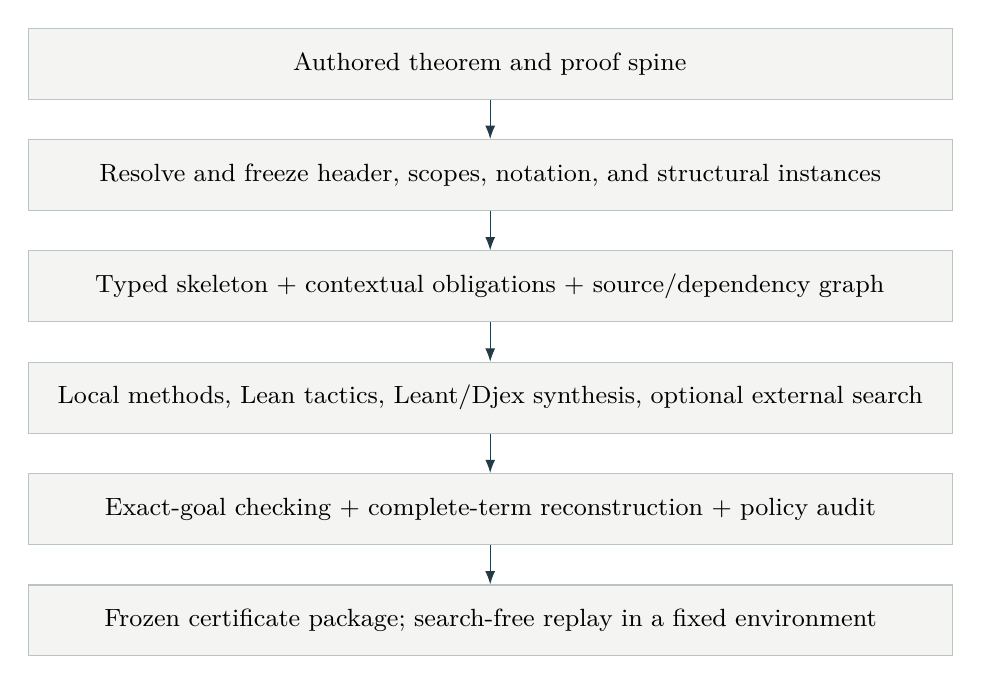
\begin{tikzpicture}[node distance=5mm,>=Latex,
 b/.style={draw=rulegray,fill=pale,rounded corners=0pt,align=center,text width=11.5cm,minimum height=9mm,font=\small},
 arr/.style={->,draw=ink}]
\node[b] (source) {Authored theorem and proof spine};
\node[b,below=of source] (header) {Resolve and freeze header, scopes, notation, and structural instances};
\node[b,below=of header] (ir) {Typed skeleton + contextual obligations + source/dependency graph};
\node[b,below=of ir] (search) {Local methods, Lean tactics, Leant/Djex synthesis, optional external search};
\node[b,below=of search] (check) {Exact-goal checking + complete-term reconstruction + policy audit};
\node[b,below=of check] (artifact) {Frozen certificate package; search-free replay in a fixed environment};
\draw[arr] (source)--(header);\draw[arr] (header)--(ir);
\draw[arr] (ir)--(search);\draw[arr] (search)--(check);
\draw[arr] (check)--(artifact);
\end{tikzpicture}
\caption{Discovery is replaceable. Statement identity, scope, and certificate acceptance are not.}
\label{fig:pipeline}
\end{figure}

A compiler should not intermingle these phases so freely that search can reinterpret the target. Bidirectional elaboration is still useful within a step: the expected type constrains omitted arguments, and known argument types constrain local expressions. What is forbidden is changing already-approved mathematical meaning because a solver found a convenient alternate reading.

\subsection{Method descriptors}
A domain method should expose a machine-readable descriptor: a stable identifier, applicability pattern, required mathematical structures, declared input facts, an obligation generator, and a checked reconstruction path. Its human documentation should state what decisions it makes automatically and what it will never infer.

For example, \code{finite_sum(split_last, combine)} recognizes an equality involving compatible finite ranges and creates endpoint and pointwise obligations. \code{continuity} recognizes a limit of a composed expression and asks for inner convergence and outer continuity. \code{surviving_terms} requires an additive map and a finite support analysis. The same descriptor gives the editor a vocabulary for failure messages and an evaluator a precise unit of functionality to test.

A method may be implemented by an ordinary Lean tactic, a custom elaborator, a proof-producing decision procedure, or an external synthesizer. The descriptor is not evidence that the implementation is correct. Each successful application must supply a reconstruction term or a certificate whose checker establishes its exact result.

\subsection{A staged local search policy}
A sensible default policy starts with predictable local work: elaboration and definitional conversion; approved simplification and context projections; direct theorem matching against supplied facts; domain methods; and then bounded search. Arithmetic, algebra, continuity, and structural propositional goals go to different engines rather than to a single indiscriminate tactic chain.

Existing Lean facilities are natural backends. Depending on the goal, a profile can use \code{simp}, \code{ring}, \code{omega}, \code{linarith}, \code{fun_prop}, Aesop, or \code{grind}. Aesop already offers user-directed best-first search and normalization, while Lean's documented \code{grind} is designed to combine cooperating forms of reasoning~\cite{aesop,lean-tactics,lean-grind}. \Spine{} should compose with these tools instead of reimplementing their mathematics.

The boundary between routine and exploratory search is a policy choice. A project might allow a small bounded proof search automatically after each \code{fact}, but require explicit approval before invoking a broad theorem retriever or a language model. The distinction controls latency and predictability, not logical soundness.

\subsection{Shared metavariables require coordinated search}
Independent-looking goals can share unknown terms. Suppose one obligation asks for a witness $x$ and two others prove $P(x)$ and $Q(x)$. It is invalid to solve them independently with incompatible witnesses and then combine their success flags. Candidate solutions must live in a common typed substitution state, or carry explicit substitutions which can be checked for compatibility.

A practical design groups obligations by shared metavariables. Parallel workers search immutable snapshots; each returns a candidate term plus its proposed substitution. The coordinator checks compatibility before committing a result and cancels or restarts affected work. Once a data choice is approved, its dependents are rechecked under the chosen value. Aesop's treatment of metavariables shared across goals is relevant prior work here, rather than evidence that this difficulty is new~\cite{aesop}.

\subsection{Contextual lemma retrieval}
Retrieval should use types and local mathematical roles, not only names or text similarity. A query includes the target's head symbols, its expected shape, the available hypotheses, and the selected profile. A result is a candidate declaration together with a proposed instantiation and the residual obligations that application would create.

A human might ask for a theorem saying that a continuous function preserves a sequence limit. The system can retrieve a suitable theorem without requiring the author to know its namespace or exact binder order. But the accepted result records the actual declaration, explicit instantiations, and resulting hypotheses. A vague description is a search request, not a theorem reference in a frozen certificate.

Locality matters for explanation as well as efficiency. The first search should try the facts the author cited and their approved structural consequences. Broadening the context can be offered as a visible suggestion: ``This step can be solved after adding theorem $L$.'' It should not quietly turn a carefully structured argument into an application of a distant theorem equivalent to the result.

\subsection{Cost models should reward useful proofs, not only short strings}
The system can rank candidate completions by a vector of costs:
\[
 (\text{new dependencies},\ \text{unapproved data choices},\
 \text{replay cost},\ \text{certificate size},\ \text{display complexity}).
\]
Unapproved choices are a hard constraint where they affect meaning, not a small numerical penalty. Other components can be selected by a project policy or exposed as Pareto alternatives. A proof using familiar local facts may be preferable to a shorter term depending on a large imported theorem. A somewhat larger reflected certificate may replay faster than a compact but expensive reduction.

This is also why a raw token count is a poor objective for the authored layer. Deleting a useful intermediate assertion can make a proof shorter and harder to maintain. The author should be able to mark a step as an explanatory boundary that proof optimization preserves.

\section{What to reuse from Leant, and what must be added}
\label{sec:leant}
\subsection{The observed design already respects several important boundaries}
The inspected Leant sources support an architecture in which a Lean goal is elaborated, translated into a synthesis fragment, searched by Djex, rendered back into candidate terms, and checked against the exact original goal. Its README also describes a tactic-by-tactic proof mode with checked suggestions and a final theorem registration step~\cite{leant-readme,fragment}.

The fragment translator is particularly instructive. Structural connectives are decomposed, while unsupported dependent and term-indexed formulas can remain opaque cargo. The source distinguishes structural information which can safely support negative conclusions from approximations for which exhausted search is inconclusive. It also distinguishes a canonical data-valued \code{Prod} from structurally similar propositions when a later behavioral adapter needs that distinction~\cite{fragment}.

These are good models for \Spine{}: preserve exact meaning outside a solver's fragment; let the solver exploit the part it understands; and never let a successful translation to a simpler language silently authorize conclusions about information that translation discarded.

\subsection{A callback receipt is not a mathematical certificate}
The source \decl{Verification.hs} defines an opaque \code{Verified candidate} wrapper. Its documentation explicitly says that this records acceptance by a supplied verification callback, not a kernel proof, solver certificate, or behavioral guarantee. Its keyed verifier also preserves the exact accepted candidate and avoids transferring authority from another occurrence merely because their rendered spellings match~\cite{verification}.

This distinction should survive in any new implementation. Useful internal states include \code{Proposed}, \code{Elaborated}, \code{KernelChecked}, and \code{PolicyApproved}. They should not all be collapsed into one field named \code{verified}. A private constructor can enforce that a receipt came from the intended boundary, but it cannot replace the stronger evidence that boundary is supposed to retain.

The certificate boundary therefore needs the exact term, expected type, environment identity, and dependency audit in addition to any scheduler receipt. Rechecking a pretty-printed term can be a useful compatibility path, but printing is not an authority-preserving transformation unless the resulting term is checked again against the same target.

\subsection{The native Lean layer}
The recommended semantic owner is a project-local Lean worker. Its internal obligations use Lean expressions and local-context identities rather than printed types. Version-sensitive elaboration, metavariable handling, and proof construction live in a narrow module family such as \code{Spine/Meta/*}. This keeps the rest of the design from becoming dependent on every implementation detail of Lean's elaborator.

A first deployment can be a Lean command or tactic which parses a \Spine{} block. It benefits immediately from the current file's environment, notation, and language-server integration. A standalone Leant-style session can use the same worker through a protocol. The worker must be built with the project's selected toolchain, not whatever Lean happens to be installed globally.

The proposed module names are architectural suggestions. They are not assertions that these interfaces already exist in Leant. The current Haskell host and external Lean backend can remain useful while the semantic bridge becomes more direct.

\subsection{The external synthesis adapter}
Djex can remain a search service for supported structural fragments. The adapter sends a versioned description of a typed query, stable handles for opaque formulas, exact provider bindings, and search limits. The original Lean obligation never leaves the worker's authority. A returned candidate is reconstructed or rendered and checked there.

The adapter must preserve binder identity, nominal type heads, universe constraints relevant to reconstruction, provider instantiations, and the distinction between propositions and data. It should not manufacture a ``lossless'' flag merely because a serialization round-trip preserved the bytes of an already-lossy abstraction. Losslessness is a semantic property of the translation used for a particular conclusion.

Leant's semantic-origin and candidate-association design is directly relevant: the current internal documentation ties candidate graphs, provider bindings, rendering, and later behavioral assessment to their originating query~\cite{synth-internals}. \Spine{} should retain that discipline when attaching a search result to an authored assertion node.

\subsection{Typed sketches and incremental synthesis}
A natural extension is a sketch such as
\[
 \lambda x.\;?f\,x\,(?g\,x),
\]
or, at the mathematical level, a proof with an explicit intermediate proposition and a missing witness. The sketch identifies what the author has already decided. Synthesis fills only the permitted holes and supplies any additional proof obligations introduced by the completion.

Dependency-aware incremental search then becomes possible. If the author changes a tail bound, certificates for unrelated finite-sum identities can remain valid. If a witness changes, all obligations whose types depend on it must be invalidated. A cache key includes the typed context and expected type, not just the source span or theorem name.

A more ambitious system can learn reusable local rules from accepted completions. Such a rule is installed only with its checked theorem and applicability pattern. Learning changes which candidates are proposed; it does not create an alternative route around proof checking.

\subsection{Behavioral synthesis and counterexamples}
For data-valued synthesis, one can combine type constraints with a behavioral specification. If the target is a function $f:A\to B$ satisfying $\forall x,\,R(x,f(x))$, the strongest artifact is a pair consisting of $f$ and a proof of that specification. Testing examples or asking an SMT solver about an abstraction is useful for search, but is not the same artifact.

Leant documents a Length-based behavioral assessment layer with replay-authorized counterexamples and conservative handling of solver outcomes~\cite{leant-readme,synth-internals}. The broader integration proposed here would allow counterexample-guided sketch refinement where an appropriate semantic model exists. That is a design extension, not a claim that arbitrary dependent mathematical specifications are already handled by Leant's current behavioral layer.

A raw \code{sat} result supplies a possible model of an encoding. Before it rejects a candidate as violating the intended specification, the system must establish the relevant correspondence or replay a concrete counterexample. A raw \code{unsat} result establishes at most what the encoding and solver evidence justify. To accept a Lean theorem, reconstruct a Lean proof, or use a verified certificate checker whose soundness theorem connects the certificate to the exact proposition. Unsupported encodings and timeouts remain inconclusive.

\subsection{Negative results need a different vocabulary}
Failure to synthesize a proof is not a proof of the negation. Even a complete search for an intuitionistic propositional abstraction establishes nonderivability in that fragment, not automatically a Lean term of $\neg P$. A countermodel or metatheoretic noninhabitation argument must state the fragment and its correspondence assumptions explicitly.

A useful result type therefore distinguishes certified success, an ill-typed candidate, an unsupported translation, exhausted search bounds, a checked counterexample to a specified data property, and fragment-relative negative evidence. The latter is never silently coerced into a proof of the original proposition's negation. The conservative distinctions visible in Leant's translator should be retained, not replaced with a single attractive ``impossible'' message~\cite{fragment,leant-readme}.

\section{Trust, certificates, and reproducible verification}
\label{sec:trust}
\subsection{Proof correctness and statement fidelity are separate guarantees}
A formally valid proof can establish the wrong theorem. For example, a header might resolve a notation to an unintended operation, choose the wrong topology, or interpret a quantifier at the wrong type. No subsequent proof search can repair that semantic mismatch merely by producing a valid term.

The certificate package should therefore expose two linked records: the approved elaborated statement and the proof of it. The editor can show a compact mathematical header by default and an expanded header containing all domains, resolved structures, and assumptions on demand. A semantic diff highlights changes to that record, even when the source edit looks typographical.

An independent proof checker still proves only a statement about its input expressions. Confidence that these expressions faithfully represent the surface document comes from a small, specified front end, conservative notation rules, tests, and inspectable expansion. A future verified elaborator could strengthen that guarantee, but it should not be claimed by a prototype which merely emits Lean source.

\subsection{The trust profile is an allowlist, not a blacklist}
The minimum kernel-oriented profile rejects unresolved metavariables, placeholders, and arbitrary unapproved axioms. A mathematical project can explicitly authorize a standard classical basis, for example dependencies on \code{propext}, \code{Classical.choice}, and \code{Quot.sound}, while another project chooses a stricter basis. Actual acceptance must audit transitive dependencies, including those reached through definitions and imported theorems~\cite{lean-axioms}.

A positive allowlist is preferable to a rule that merely rejects \code{sorryAx}. Computation-backed proof mechanisms can have version-dependent trust dependencies. The Lean reference distinguishes ordinary logical axioms from compiler-trust mechanisms; their exact names and handling should be audited for the target toolchain rather than copied from an unrelated version of the manual~\cite{lean-axioms}. The inspected ProveIt snapshot uses Lean 4.32.0, whereas the live documentation consulted for this study is not a pinned description of that exact installation.

The recommended default is a kernel-replay profile: reflective computation is acceptable when a checked correctness theorem and kernel-checkable reduction establish the result. A project may separately opt into a broader native-computation trust profile. Such a choice must be visible in the artifact, not inferred from a tactic returning success.

\subsection{Imported environments are part of the claim}
The judgment $\mathcal E\vdash p:T$ is relative to $\mathcal E$. If an imported declaration is an unapproved axiom, a valid application of it does not meet a stricter trust policy. A publication-grade checker must start from approved immutable dependencies, or validate their declarations and dependency closure, before accepting the new proof.

This need not mean recompiling the entire mathematical library for every local edit. A previously validated environment can be reused by content identity. What must not happen is treating a fresh file name, an unexamined binary artifact, or a line of diagnostic output saying ``no axioms'' as sufficient authority.

The independent check should occur outside the mutable search process. A tactic or plugin can manipulate elaboration state and may execute arbitrary host code. The acceptance worker receives only the proposed proof artifacts and a manifest of expected declarations; it cannot accept an extra declaration introduced by the search process merely because that process labeled it a helper theorem. Such helpers require their own checked definitions or proofs.

\subsection{What the certificate package contains}
A certificate package should include the fixed theorem type, the completed proof term or a versioned reconstruction certificate, the exact global declaration identities needed to interpret it, and the source-node association for every asserted step. It also includes the approved trust policy, the recorded axiom closure, and any selected data witnesses or structural instances whose identity matters.

Search provenance is useful but secondary: engine versions, budgets, random seeds when relevant, and candidate ranking choices explain how the proof was found. They need not be rerun to establish its validity. In particular, changing a search engine should not invalidate an already checked proof term merely because the new engine would choose a different proof.

A schematic manifest might look like this:
\par\noindent\begin{minipage}{\linewidth}
\examplelabel{Proposed artifact manifest; fields describe identities, not proofs by themselves}
\begin{Code}
certificate-format: spine-cert/1
statement: <serialized, elaborated Lean expression>
statement-digest: <digest of that expression and its binding data>
environment: <validated dependency manifest>
toolchain: <exact Lean and library revisions>
trust-profile: <approved policy identifier and content digest>
source-nodes: <stable node ids, typed contexts, expected types>
proofs: <closed declarations or contextual proof objects>
choices: <approved data and structural choices>
provenance: <optional search runs and reconstruction diagnostics>
\end{Code}
\end{minipage}\par\smallskip
A digest protects identity and cache coherence; it does not make an untrusted declaration true. Serialization also needs validation: malformed references, duplicate identifiers, cyclic declaration dependencies, and inconsistent universe data must be rejected before checking.

\subsection{Frozen replay versus exploratory reconstruction}
There should be two explicit operational modes. In exploration mode, a missing or stale certificate triggers local reconstruction under the selected search budget. In frozen mode, the checker validates the supplied terms and manifests and reports stale or missing artifacts; it does not silently launch a different search and substitute a new proof.

Frozen replay is deterministic relative to the fixed checker, proof objects, and dependency environment. It does not promise byte-identical artifacts across arbitrary compiler versions. A Lean upgrade is a migration event: rebuild or translate the certificate representation, recheck the terms and dependencies, and expose any changed statement resolution. Storing an \code{.olean} file alone is not a universal cross-version certificate format.

For a first implementation, an export of explicit Lean declarations with independently fixed types can be a practical intermediate format. Re-elaboration may still be needed, but heuristic proof search should be eliminated from that export. The exported terms are checked anew; their printed appearance is not treated as evidence of equivalence to an earlier in-memory term.

\subsection{Dependency controls and explanatory fidelity}
A clause such as \code{using only h1, h2} needs a precise meaning. One useful policy permits the named local facts, the foundational constants needed to state their types, and an explicit profile library. The checker then audits the accepted proof against that allowance. It should report separately the local facts actually used, the library declarations used, and the transitive axiom closure.

This is not equivalent to a string search for theorem names in the printed term. A definition can hide a theorem dependency; a cast can hide structural arguments; an imported theorem can carry an axiom. Conversely, the type of a permitted local fact can mention constants which are necessary vocabulary but not independent reasons for the inference. The policy therefore needs typed dependency categories, not one flat list of words.

Even an exact dependency audit cannot prove that an explanation is pedagogically satisfying. A proof may mention a fact in a mathematically irrelevant way, or use a powerful theorem which makes the rest of the outline unnecessary. \Spine{} can enforce that every displayed assertion is true, reveal actual dependencies, and warn about unused material. It should not claim that the kernel has certified the author's explanatory narrative.

\subsection{Incremental checking and cache locality}
The cache key for an obligation should include its typed telescope, target, fixed choices, relevant declaration identities, and acceptance policy. Alpha-renaming and irrelevant whitespace can be normalized away. Hashing only the visible goal text is unsafe; hashing the entire repository on every edit is safe but unnecessarily destructive to reuse.

A dependency-projected cache provides a better balance. Once a proof is fixed, it references exact constants, not open-ended theorem searches or namespace lookups. Under a conservative environment extension preserving those constants and its policy, the same term can be rechecked without rediscovery. Search profiles and solver versions remain provenance unless a policy specifically requires them for acceptance.

The initial implementation can use conservative whole-environment invalidation and evolve toward finer-grained reuse. Correctness comes first; cache locality is an optimization. The interface should distinguish ``proof invalid'', ``proof not yet rechecked'', and ``cache entry unusable'' rather than displaying the same red error for all three.

\section{Editing experience: ask for the missing mathematics}
\label{sec:ux}
\subsection{Progressive disclosure}
The normal editor view is the proof spine. An assertion can be expanded into its generated obligations, the selected library theorems, and the completed Lean term. A second expansion exposes coercions, structural instances, and dependency details. The reader should not need to expand everything to know the theorem's assumptions or whether a step is checked.

A useful status model distinguishes a certified node, an unresolved node, a stale node, and a failed candidate attempt. A failed search does not mark the mathematical assertion false. The source should remain a legible mathematical document while showing exactly where formal evidence is still missing.

This is a better use of automation than constantly rewriting the user's source into a long tactic script. Generated detail belongs in an inspectable layer; an author can promote a useful generated intermediate fact into the spine when it clarifies the argument.

\subsection{Diagnostics should name obligations, not implementation accidents}
For the convolution calculation, a useful message is:
\begin{quote}
To normalize the natural subtraction in this summand, the method needs $m\le n$. The current branch permits $m=n+1$. Split the endpoint from the residual sum or handle this branch separately.
\end{quote}
For the formal-root application:
\begin{quote}
The formal implicit-root theorem requires the linear coefficient to be a unit of $R$. The available fact proves only that it is nonzero. These conditions are not equivalent for the declared commutative ring.
\end{quote}
For the contraction argument:
\begin{quote}
The proposed orbit limit requires $|q|<1$. The current assumption is $|q|\le1$; the geometric-decay method does not cover the boundary.
\end{quote}
These messages follow from a method's contracted obligations. They are not attempts to infer intent from a low-level elaborator exception after the fact.

\subsection{Counterexamples as local debugging aids}
When an arithmetic side condition is false, a small concrete counterexample is often more helpful than a failed tactic. The natural-subtraction example $n=0,m=1$ and the integer-ring example $2s_1=1$ are informative because they explain the mathematical mismatch.

A counterexample tool must label its scope. It may refute a proposed local rewrite or a specific candidate witness without refuting the original theorem, which might have another proof. For example, failure of a uniform contraction estimate does not show that two particular probability measures differ. The diagnostic should attach the counterexample to the exact obligation it addresses.

\subsection{Suggestions should change the right layer}
There are at least three different suggestions an editor can make: fill a local proof hole; add a missing hypothesis or change a theorem statement; or change the proof strategy. They should be presented differently. The first can often be accepted as generated detail. The second changes the mathematical claim and requires explicit review. The third changes the authored proof spine, such as replacing double induction with the triangular-sum argument.

A language model can be useful at all three levels, but its output must identify which kind of edit it proposes. In particular, an automatic repair must not quietly weaken the theorem and then report the original task as completed.

\subsection{Round trips, escape hatches, and mixed developments}
The initial language should coexist with ordinary Lean. A \code{by lean \{ ... \}} block can supply a proof term through familiar tactics, subject to the same statement and trust checks. Generated terms can be exported for debugging. Existing Lean lemmas can be referenced directly without wrappers, while project-local aliases provide readable names for frequently used interfaces.

An escape hatch should bypass convenience syntax, not verification. It cannot introduce unapproved axioms, change the frozen header, or certify an unresolved node. Conversely, the new language should not force users to reproduce a concise existing Lean proof in more verbose prose merely to satisfy a stylistic convention.

\section{Relationship to existing proof languages and automation}
\label{sec:prior}
The broad idea of writing readable, declarative formal proofs is established, not a novelty claim of this proposal. Isar explicitly targets structured, intelligible proof documents with integrated proof methods; Mizar develops a formal language close to mathematical vernacular~\cite{isar,mizar}. \Spine{} should learn from their emphasis on readable structure rather than rediscover it under a new name.

Naproche studies controlled mathematical language and its translation into proof-oriented representations, including nested assumption scopes~\cite{naproche}. This supports the decision to treat discourse structure as semantic data. The present proposal chooses a narrower initial front end: typed Lean expressions plus a controlled proof grammar, rather than unrestricted mathematical English.

Verbose Lean is especially close as an implementation precedent. Massot describes a Lean-based controlled-natural-language library designed to help students move between formal proofs and traditional written mathematics~\cite{verbose}. The purpose here differs in emphasis: the target user is an experienced mathematician or formalizer, and the central problems are representation transport, synthesis boundaries, and stable certificates for research-scale developments. That difference does not imply that a separate language is always preferable to a library extension.

Aesop addresses predictable, user-configurable proof search and already handles important complications such as shared metavariables~\cite{aesop}. It is a backend and a source of implementation lessons, not something \Spine{} should replace. Lean's native tactics and \code{grind} similarly reduce the marginal value of merely inventing a new word for ``try automation''~\cite{lean-tactics,lean-grind}.

Recent proof-refactoring research also treats proof length, checking cost, and other objectives jointly. For example, the 2026 \emph{Lean Refactor} preprint studies agentic, multi-objective optimization of existing Lean proofs~\cite{lean-refactor}. This is another reason that the correct comparison is not only against untouched source files. Better ordinary Lean is a serious baseline.

\begin{table}[htbp]
\centering\small
\begin{tabularx}{\textwidth}{@{}p{.25\textwidth}XX@{}}
\toprule
Approach & Lesson to retain & Emphasis of this proposal\\
\midrule
Isar and Mizar & Declarative structure and readable arguments & Contextual reconstruction of representation detail\\
Naproche & Mathematical discourse has formal scope & Typed expressions and a narrow initial grammar\\
Verbose Lean & Lean can host a mathematical proof surface & Research-scale methods and stable evidence layers\\
Aesop and Lean tactics & Reuse mature proof-producing automation & Contracted steps and explicit discovery boundaries\\
Leant and Djex & Type-directed synthesis with exact-goal checks & Persistent obligations and certificate ownership\\
Proof refactoring & Multiple objectives and strong Lean baselines & Preserve authored mathematical choices\\
\bottomrule
\end{tabularx}
\caption{Complementary precedents. The intended contribution is their source-driven integration, not the invention of declarative proof or certified automation.}
\end{table}

The distinctive design hypothesis is therefore modest and testable: a persistent layer of typed mathematical steps, each connected to explicit local obligations and frozen completion evidence, can make difficult proofs easier to write and maintain than either raw tactic scripts or opaque one-shot automation. The case studies motivate that hypothesis; they do not yet measure its success.

\section{An implementation plan organized around vertical slices}
\label{sec:implementation}
\subsection{First slice: a small Lean-native core}
The first usable implementation should support theorem headers, \code{take}, \code{assume}, \code{let}, \code{fact}, \code{show}, and \code{calc}. It should reuse Lean's mathematical expression parser and elaborate into ordinary terms. A bounded local solver fills assertion holes. The editor shows residual obligations and the generated terms. The exporter rejects every unresolved hole and performs the configured dependency audit.

This slice is valuable even without external synthesis. It establishes source identity, contextual obligations, statement freezing, and a checkable artifact. Those foundations should be tested before adding ambitious proof search, because otherwise a later success can mask an incorrect ownership or scope model.

The implementation need not initially invent a compact binary certificate format. Explicit generated Lean declarations and a source-node manifest are sufficient to test the workflow, provided replay is honest about re-elaboration and uses the fixed expected types.

\subsection{Second slice: the finite-sum case study}
Implement bounded-domain binders, endpoint splitting, sum congruence, natural-arithmetic guard propagation, and a small set of certified finite-index views. Add Pascal as an ordinary registered theorem. Reproduce the same-plan convolution proof and the odd-prefix cancellation example.

This slice should have strong negative tests. Move the endpoint into the residual branch; change inclusive bounds to exclusive bounds; remove the bound required for a subtraction rewrite; change the coefficient ring; and alter an index map so it is no longer bijective. Failures should be local and intelligible, not discovered only when the final large term is assembled.

Do not add a universal ``simplify mathematics'' method to make the showcase pass. The purpose is to validate that a small method vocabulary can account for the actual proof obligations observed in the source.

\subsection{Third slice: iteration and limits}
Add an iteration schema with an explicit orbit, a continuity-composition schema, and order passage to a limit. Reproduce the characteristic-function proof without changing its mathematical hypotheses. The ambient space bundle must elaborate to the exact collection of source-compatible structures, and the replayed theorem header must be compared with the baseline.

Tests should include $q=0$, a negative $q$ with $|q|<1$, an invalid boundary assumption $|q|\le1$, and a one-step inequality stated only at a single point. These distinguish mathematical generality from accidental behavior of a particular proof script.

\subsection{Fourth slice: coefficient views and surviving support}
Introduce typed polynomial and formal-series coefficient notation, homomorphism transport, and the surviving-terms method. Reproduce the constant-coefficient theorem and apply the existing generic formal-root theorem. The odd/even branch context and the unit hypothesis are explicit acceptance tests.

Only after these slices work should the system generalize the methods into a larger domain library. Generalization should be driven by additional proofs, not by a speculative ontology of every mathematical phrase.

\subsection{Fifth slice: Leant integration and richer synthesis}
Connect the fixed obligation interface to Leant/Djex search. Start with propositional and higher-order structural plumbing, where the inspected architecture is directly relevant. Preserve source-origin records and exact candidate identity through rendering and checking. Add typed sketches and data specifications only with tests demonstrating that the extra semantic requirements are actually enforced.

Broad theorem retrieval, language-model suggestions, and SMT-guided behavioral search can then be layered on as replaceable discovery components. They should not require changes to the certificate checker or to the meaning of existing source nodes.

\subsection{A deliberately small trusted surface}
Most convenience machinery should be untrusted proof construction. Domain methods can be large, heuristic, or user-defined because their outputs must be checked. The parts deserving the strongest engineering attention are statement resolution and display, contextual substitution, artifact loading, dependency auditing, and independent proof validation.

The first implementation should also document its limitations precisely. For example, it might support finite reindexing but not dependent quotient transport, or sequences in normed spaces but not general filters. An explicit supported fragment is preferable to an impressive surface which silently delegates every difficult semantic decision to an opaque agent.

\section{How to evaluate the design without flattering it}
\label{sec:evaluation}
\subsection{Fix the theorem, the environment, and the proof-plan category}
The first benchmark should use the inspected declarations as a development set, then add held-out theorems from unrelated files and domains. The theorem being proved, its statement, and the permissible environment are frozen. The original target declaration and any downstream theorem that leaks its proof are unavailable to the solver. A dependency audit checks that a ``compressed'' proof has not simply imported the answer.

At least three proof-plan categories should be reported separately: same plan and same library; a changed proof plan using the same library; and a changed library with newly factored helper theorems. The double-induction and triangular-sum proofs illustrate why these categories cannot be mixed.

The comparison should include untouched Lean, human-refactored Lean, ordinary Lean with the same improved helper library, applicable existing automation, and the proposed \Spine{} surface. A language-model-generated Lean proof is another useful baseline when the same model is allowed to propose \Spine{} proofs. Otherwise the evaluation might attribute a better search agent to a better language.

\subsection{Measure author work, not just source size}
Useful outcomes include time to first checked proof, time to repair a deliberately broken proof, number of manually supplied mathematical facts, and the number of library-specific adapters the author had to write. Source lines and tokens can be reported, but they are supplementary.

Generated evidence has costs too: proof-object size, peak checking memory, replay latency, and sensitivity to library upgrades. An apparent reduction in authored text can be a poor trade if every small edit causes minutes of unbounded search or produces an enormous term. Report distributions, especially tail latency, rather than only averages.

Readability should be evaluated by tasks: identify the induction invariant, explain why a denominator is nonzero, find the hypothesis needed for a limit, or locate the step invalidated by a changed assumption. A reader's success on those tasks is more informative than whether a proof visually resembles prose.

\subsection{Charge for displaced complexity}
Every newly introduced helper theorem, profile, and domain-specific method has a cost. Some of that cost is amortized across many proofs; that is the point of a library. The evaluation should show both the initial development cost and the marginal author effort once the method is available.

A fair compactness report might therefore give three quantities: authored proof size, newly added reusable mathematical material, and generated certificate size. These cannot simply be added as if they had identical value, but displaying all three prevents an implausible claim that complexity has vanished because it moved to another file.

The already-short \decl{existsUnique_germRoot} and forward-difference proofs are useful negative controls. A system that makes them longer or more fragile should acknowledge that regression and allow ordinary Lean to remain the better surface for those cases.

\subsection{Adversarial semantic tests}
The following tests should be part of the design's acceptance criteria. They are proposed tests, not a claim that an implementation has passed them.
\begin{longtable}{@{}p{.31\textwidth}p{.63\textwidth}@{}}
\toprule
Mutation or attack & Required behavior\\
\midrule
\endfirsthead
\toprule
Mutation or attack & Required behavior\\
\midrule
\endhead
Natural subtraction outside its guard & Reject the invalid transport or split cases; expose $n=0,m=1$ as a local counterexample when applicable.\\[4pt]
Endpoint merged with residual sum & Do not reuse $m\le n$ in the $m=n+1$ branch.\\[4pt]
Evenness removed from $m/2>0$ & Do not infer positivity from $m\ne0$ alone.\\[4pt]
Unit weakened to nonzero over $\Z$ & Leave the implicit-root unit obligation unsolved; do not import a field-only theorem.\\[4pt]
$|q|<1$ weakened to $|q|\le1$ & Reject the generic geometric-decay step at the boundary.\\[4pt]
Finite sum changed to infinite sum & Demand the hypotheses of an applicable infinite-sum interchange theorem.\\[4pt]
Witness moved before its dependency & Reject an out-of-scope reference rather than changing the quantifier order.\\[4pt]
Branch assumption used in a sibling & Reject the scope map or the resulting term.\\[4pt]
Hidden arbitrary axiom in a helper & Reject under the kernel-replay allowlist after transitive dependency inspection.\\[4pt]
Same text, different source identity & Preserve the exact accepted candidate's authority; do not transfer a receipt by spelling alone.\\[4pt]
Changed topology or coefficient ring & Invalidate affected statements and certificates, even if the pretty-printed header is similar.\\[4pt]
Solver returns \code{unknown} or times out & Report an inconclusive search outcome, not a proof or a refutation.\\[4pt]
Formal root used as an analytic function & Generate separate convergence and interpretation obligations.\\[4pt]
Unused false intermediate assertion & Refuse document certification even if another route proves the final theorem.\\
\bottomrule
\end{longtable}

\subsection{Stability tests and a realistic success criterion}
Add an irrelevant lemma to an imported module, rename a bound variable, alter only comments, or change a search engine's ranking. Frozen proof terms should remain checkable whenever their actual semantic dependencies and policies are unchanged. Conversely, changing a relevant definition or a structural instance should invalidate the affected evidence rather than reuse an attractive but stale cache entry.

A convincing early result would not be ``all proofs become one line''. It would be that, on held-out proofs with the same mathematical content, authors write fewer representation adapters, diagnose missing hypotheses more quickly, and obtain stable checking behavior, while the generated terms and dependency audits preserve the original theorems. That is an engineering and mathematical usability claim which can actually be tested.

\section{The recommended design in one argument}
The inspected ProveIt proofs suggest that a large part of practical verbosity lies between the mathematical proof idea and the library's chosen representation. Leant shows that typed synthesis can operate across that gap without giving the search engine final authority, provided exact goals, candidate identity, and the strength of evidence are carefully preserved~\cite{prefix,affine,germ,fragment,verification}.

The right abstraction is therefore not ``English instead of Lean''. It is a persistent layer of \emph{typed mathematical intent}: choose the orbit; specify the induction motive; name the finite region; identify the surviving terms; apply a theorem through its mathematical contract. Each instruction expands to explicit contextual obligations, and every completed obligation contributes a checkable term.

The author should not have to choose a congruence combinator merely to compare matching summands. The author should still choose which sums to compare. The author should not have to spell out lambda composition merely to use continuity. The author should still supply the limiting argument and the relevant continuity hypothesis. The author should not manually shuttle between \code{Fin} and \code{Finset} when an approved equivalence is already known. The system should still prove that the shuttle preserves the expression being used.

\begin{principle}{The practical recommendation}
Build \Spine{} first as a Lean-native proof layer with a small core and a few source-driven domain methods. Reuse Lean's existing automation and Leant/Djex's synthesis where they fit. Freeze the statement before search, keep source assertions individually accountable, and separate generated proof evidence from discovery transcripts. Expand the language only when a new mathematical pattern justifies a new contract.
\end{principle}

This direction offers a plausible route to proofs which are both closer to a mathematician's reasoning and no less explicit at the point where explicitness matters: the object ultimately checked by the kernel.

\appendix
\section{A compact core grammar and extension boundary}
\label{app:grammar}
The following grammar is intentionally a core rather than a complete concrete-syntax specification. Indentation and brackets delimit blocks; \code{term} and \code{type} refer to the host mathematical expression grammar. Domain-specific display forms desugar to these nodes before proof search.
\par\noindent\begin{minipage}{\linewidth}
\begin{Code}
declaration ::= theorem name parameters ":" type proof
proof       ::= "proof" ["using" profile-list] block "end"
block       ::= statement*
statement   ::= "take" binder
              | "assume" name ":" term
              | "let" name parameters ":=" term
              | "fact" name parameters ":" term justification
              | "show" term justification
              | "suffices" term justification
              | "choose" binder "with" name "from" term
              | "cases" term ":" case-blocks
              | "induct" name ["generalizing" names] ":" case-blocks
              | "calc" calculation
justification ::= "by" method ["using" dependency-list]
                | "by" proof
method      ::= registered-method arguments
              | "lean" "{" host-proof "}"
\end{Code}
\end{minipage}\par\smallskip
The grammar alone does not authorize every statement in every goal. Elaboration checks the expected connective, eliminator, binder domain, and target sort. For example, \code{take} introduces a universal binder; it is not an arbitrary existential choice. \code{choose ... from ...} eliminates evidence; it does not ask unrestricted synthesis to invent a witness.

Method combinators such as \code{then} compose refinements of generated obligations. Their exact goal-selection policy must be specified: all generated goals, a named obligation, or the unique residual goal. Implicitly applying a continuation to whichever goal happens to be first recreates a major source of tactic-script fragility. Stable obligation identities are preferable to positional goal numbering.

The domain notation used in the examples---bounded sums, \code{retain only}, coefficient paths, and sequence-limit sentences---is presentation syntax for ordinary expressions and core proof nodes. A parser extension supplies both its expansion and the information needed to display that expansion faithfully. A formatter is required to preserve the typed node, not merely produce pleasant prose.

\section{Implementation invariants and a candidate-acceptance sketch}
\label{app:algorithm}
A minimal implementation should make the following invariants executable. The theorem header never changes after approval. Every obligation has one authoritative expected type and context. Every candidate retains the identity of the query from which it arose. Every asserted source node must be certified before publication. No raw solver verdict is a proof object. No unresolved hole is exported as a theorem parameter or an axiom.

The acceptance logic can be expressed in implementation-neutral pseudocode:
\par\noindent\begin{minipage}{\linewidth}
\begin{Code}
accept(obligation, proposal, immutable_environment):
    require proposal.origin matches obligation.identity
    require obligation.statement is still current
    require proposal.scope_map is well-formed

    isolated := create_check_context(immutable_environment,
                                     obligation.telescope)
    term := reconstruct(proposal, expected=obligation.target,
                        context=isolated)
    term := instantiate_only_approved_substitutions(term)

    reject if term contains unresolved metavariables
    reject if term refers to unavailable local variables
    reject if reconstruction introduced unapproved declarations
    require kernel_check(term, obligation.target, isolated)
    require dependency_policy_accepts(term, obligation.policy)

    return certificate(term, obligation, actual_dependencies(term))
\end{Code}
\end{minipage}\par\smallskip
The final theorem assembler performs another check after substitution of all local certificates. The dependency auditor examines the transitive declarations required by the accepted term under the chosen policy; it does not trust a dependency list supplied by the search engine.

Reconstruction itself may fail or time out, and a well-typed term may be rejected by policy. Those outcomes should remain distinct in diagnostics. A checked term which exceeds a preferred size budget is not logically invalid; a project can treat size as an artifact-quality gate without mislabeling it as a mathematical error.

An efficient implementation can share expression DAGs and validated dependency closures. Nevertheless, no linear-time verification claim follows merely from DAG sharing. Definitional reduction and proof reconstruction can be expensive. Actual checking time and memory must be measured for the chosen certificate representation and Lean version.

\section{Source manifest and limits of the review}
\label{app:sources}
\subsection{ProveIt}
All ProveIt source references below use commit
\begin{center}\code{24ce8bd743eaab64a91ce90725ea00f498d319d2}.\end{center}
The root \code{lean-toolchain} was read and selects \code{leanprover/lean4:v4.32.0}. The three case-study files are under
\begin{center}\code{Analysis/FabiusFunction/Lean/FabiusFunction/}.\end{center}

\begin{longtable}{@{}p{.34\textwidth}p{.60\textwidth}@{}}
\toprule
File and inspected range & Declarations used in this article\\
\midrule
\endfirsthead
\toprule File and inspected range & Declarations used in this article\\\midrule
\endhead
\decl{ThueMorsePrefix.lean}\newline Lines 1--230 &
\decl{iteratedPrefix}; \decl{iteratedPrefix_at_zero}; \decl{iteratedPrefix_succ_sub}; \decl{iteratedPrefix_one_two_mul_add_one}; \decl{iteratedPrefix_convolution}; \decl{iteratedPrefix_eq_sum_kernel}.\\[6pt]
\decl{AffineIndependentCopy.lean}\newline Lines 1--220 &
\decl{affineIndependentCopyLaw_isProbabilityMeasure}; \decl{charFun_iterate_of_affineIndependentCopy_fixedPoint}; \decl{eq_of_charFun_affine_recurrence}; \decl{affineIndependentCopyLaw_fixedPoint_unique}.\\[6pt]
\decl{AlgebraicInverseGerm.lean}\newline Lines 1--210 &
\decl{evenWeightSeries}; \decl{germPolynomial}; \decl{constantCoeff_coeff_germPolynomial}; \decl{existsUnique_germRoot}; \decl{germRoot}; \decl{germPolynomial_eq_sum}; the dyadic quadratic instance.\\
\bottomrule
\end{longtable}
Long identifiers in this manifest may wrap typographically; the linked source files preserve their exact spelling. Other repository directories and import surfaces were inspected for orientation, but the mathematical review claims are limited to the declarations and ranges above. Imported theorems were used as the interfaces shown by these source proofs, not independently re-audited throughout their dependency closure.

\subsection{Leant}
All pinned Leant references use commit
\begin{center}\code{3a40904be8a410d832d9ab6900b3d3e7b425eccb}.\end{center}
The inspected sources include \decl{src/Leant/Synth/Fragment.hs}, lines 1--235, and \decl{src/Leant/Synth/Verification.hs}, lines 1--260. The pinned README section at lines 330--520 was read, along with the earlier README overview and the opening source-boundary sections of \code{docs/synth-internals.md}. These establish the structural synthesis, proof-suggestion, exact-candidate, and evidence distinctions discussed in the text.

The article does not claim a complete audit of \code{Engine.hs}, \code{Render.hs}, the external solver implementation, or Leant's entire backend lifecycle. Integration interfaces proposed here are design recommendations. Test counts reported in the repository documentation were not rerun and are not presented as experimental results of this study.

\subsection{Validation status of the deliverable}
The mathematical proofs in Sections~\ref{sec:prefix-case}--\ref{sec:germ-case} and the conditional completion argument in Section~\ref{sec:semantics} are expository derivations. They have not been compiled as \Spine{} or independently formalized for this article. The code blocks explicitly labeled existing Lean are excerpts from the inspected sources (with the neighborhood notation expanded to \code{nhds} in one listing); the remaining language examples and algorithms are specifications or pseudocode.

The accompanying source is self-contained LaTeX with an embedded bibliography. The PDF was built from that source. The included README specifies the build procedure and the distinction between a typeset design study and an implemented proof-language toolchain.

\clearpage
\phantomsection
\addcontentsline{toc}{section}{References}
\begin{thebibliography}{99}
\small\raggedright
\bibitem{prefix}
Vladimir Reshetnikov et al.
\textit{ProveIt: ThueMorsePrefix.lean}.
Snapshot \code{24ce8bd743eaab64a91ce90725ea00f498d319d2}, inspected lines 1--230.
\srcp{Analysis/FabiusFunction/Lean/FabiusFunction/ThueMorsePrefix.lean}{Pinned source on GitHub}.

\bibitem{affine}
Vladimir Reshetnikov et al.
\textit{ProveIt: AffineIndependentCopy.lean}.
Same ProveIt snapshot, inspected lines 1--220.
\srcp{Analysis/FabiusFunction/Lean/FabiusFunction/AffineIndependentCopy.lean}{Pinned source on GitHub}.

\bibitem{germ}
Vladimir Reshetnikov et al.
\textit{ProveIt: AlgebraicInverseGerm.lean}.
Same ProveIt snapshot, inspected lines 1--210.
\srcp{Analysis/FabiusFunction/Lean/FabiusFunction/AlgebraicInverseGerm.lean}{Pinned source on GitHub}.

\bibitem{toolchain}
Vladimir Reshetnikov et al.
\textit{ProveIt: lean-toolchain}.
Same ProveIt snapshot.
\srcp{lean-toolchain}{Pinned toolchain selection on GitHub}.

\bibitem{leant-readme}
Vladimir Reshetnikov et al.
\textit{Leant: README, interactive proving and automatic term synthesis}.
Snapshot \code{3a40904be8a410d832d9ab6900b3d3e7b425eccb}.
\srcl{README.md}{Pinned README on GitHub}.

\bibitem{fragment}
Vladimir Reshetnikov et al.
\textit{Leant: src/Leant/Synth/Fragment.hs}.
Same Leant snapshot, inspected lines 1--235.
\srcl{src/Leant/Synth/Fragment.hs}{Pinned translator source on GitHub}.

\bibitem{verification}
Vladimir Reshetnikov et al.
\textit{Leant: src/Leant/Synth/Verification.hs}.
Same Leant snapshot, inspected lines 1--260.
\srcl{src/Leant/Synth/Verification.hs}{Pinned verification-boundary source on GitHub}.

\bibitem{synth-internals}
Vladimir Reshetnikov et al.
\textit{Leant: Synthesis internals}.
Same Leant snapshot; opening sections on fragment search, semantic origin, candidate authority, and Length handoff.
\srcl{docs/synth-internals.md}{Pinned documentation on GitHub}.

\bibitem{lean-tactics}
The Lean development team.
\textit{The Lean Language Reference: Tactic Reference}.
Live documentation consulted September 5, 2026; not a frozen specification of ProveIt's selected toolchain.
\url{https://lean-lang.org/doc/reference/latest/Tactic-Proofs/Tactic-Reference/}.

\bibitem{lean-grind}
The Lean development team.
\textit{The Lean Language Reference: The grind Tactic}.
Live documentation consulted September 5, 2026.
\url{https://lean-lang.org/doc/reference/latest/The--grind--tactic/}.

\bibitem{lean-axioms}
The Lean development team.
\textit{The Lean Language Reference: Axioms}.
Live documentation consulted September 5, 2026.
\url{https://lean-lang.org/doc/reference/latest/Axioms/}.

\bibitem{aesop}
Jannis Limperg and Asta Halkjær From.
\textit{Aesop: White-Box Best-First Proof Search for Lean}.
Proceedings of CPP 2023, 14 pages.
DOI: \href{https://doi.org/10.1145/3573105.3575671}{10.1145/3573105.3575671}.
\url{https://people.compute.dtu.dk/ahfrom/aesop-camera-ready.pdf}.

\bibitem{isar}
Markus Wenzel and the Isabelle project.
\textit{Isar: Intelligible Semi-Automated Reasoning}.
Project description and primary-publication index, including Wenzel's 1999 Isar paper.
\url{https://isabelle.in.tum.de/Isar/}.

\bibitem{mizar}
The Mizar project.
\textit{Mizar Language}.
Primary project description.
\url{https://mizar.uwb.edu.pl/language/}.

\bibitem{naproche}
M. Cramer, P. Koepke, D. Kühlwein, B. Schröder, and J. Veldman.
\textit{The Naproche Project: Controlled Natural Language Proof Checking of Mathematical Texts}.
CEUR Workshop Proceedings, vol. 448, 2009.
\url{https://ceur-ws.org/Vol-448/paper10.pdf}.

\bibitem{verbose}
Patrick Massot.
\textit{Teaching Mathematics Using Lean and Controlled Natural Language}.
ITP 2024, LIPIcs 309, article 27, pp. 27:1--27:19.
DOI: \href{https://doi.org/10.4230/LIPIcs.ITP.2024.27}{10.4230/LIPIcs.ITP.2024.27}.
\url{https://drops.dagstuhl.de/entities/document/10.4230/LIPIcs.ITP.2024.27}.

\bibitem{lean-refactor}
Jialin Lu, Soonho Kong, Rodrigo Stehling, Kaiyu Yang, Zhangyang Wang, Weiran Sun, and Wuyang Chen.
\textit{Lean Refactor: Multi-Objective Controllable Proof Optimization via Agentic Strategy Search}.
arXiv:2605.20244, 2026. Preprint; cited for the optimization problem and proposed approach, not as a benchmark of \Spine{}.
\url{https://arxiv.org/abs/2605.20244}.
\end{thebibliography}
\end{document}
